\documentclass[a4paper, 12pt]{article}
\author{Justin Clough, RIN:661682899}
\title{FEP Assignment 4}
\usepackage{geometry}
\usepackage{float}
\usepackage{subfigure}
\usepackage[justification=centering]{caption}
\usepackage{enumerate}
\usepackage{multirow}
\usepackage{listings}
\lstset{
    escapechar=`,
    language=C++,
    numbers=left,
    tabsize=2,
    prebreak=\raisebox{0ex}[0ex][0ex]{\ensuremath{\hookleftarrow}},
    frame=single,
    breaklines=true,
}
\usepackage{graphicx}
\graphicspath{ {images/} }
\usepackage{nameref}
\usepackage{amsmath}
\usepackage{amssymb}
\usepackage{amsfonts}
\usepackage[linesnumbered,ruled]{algorithm2e}
\usepackage{tikz}
\usetikzlibrary{calc,patterns,decorations.pathmorphing,decorations.markings,positioning,automata}
\usepackage{pgfplots}
\usepackage{pgfplotstable}
\usepackage{makecell}

\begin{document}
\maketitle

\newpage
\section{Introduction} \label{sec:intro}
The purpose of this project was to develop a Finite
Element Analysis (FEA) code that solves linear
elliptic problems. This project does so for
two dimensional plane stress solid mechanic problems. The user
provides the code with the following information
(an example input script is shown in
Appendix \ref{subsec:ExIn}):

\begin{itemize}
  \item A geometric model of the domain in the
        form of a \emph{.dmg} file.
  \item The corresponding mesh of the domain in the
        from of a \emph{.smb} file.
  \item An associations file which define geometric
        node sets in the form of a \emph{.txt} file. The
        details of this file are explained in detail in
        section \ref{sec:codeDes}.
  \item A control file which define material properties,
        boundary conditions, and linear algebra details in
        the form of a \emph{.yaml} file.
  \item A file name to write the solution to as an array of
        characters.
  \item The order of numerical integration as an integer.
  \item The body load in the form of three floating point
        number.
\end{itemize}

Based on these input parameters, the code assembles and
solves the relevant finite element problem to retrieve
the displacement at each mesh Degree of Freedom (DOF).
It then calculates the Cauchy stress tensor for each
integration point of each element. It finally writes
the displacement, traction, and Cauchy stress fields to
file in \emph{.vtk} format.

The rest of this report is separated into the following
section. The technical description of the code, which
includes an overview of the Finite Element Method (FEM),
the numerical integration techniques used, and the
linear algebra assembly and solution methods is shown in
section \ref{sec:techDes}. A description of the code, which
includes an outline of classes created and a pseudo code
is shown in section \ref{sec:codeDes}. The tests performed
are described in section \ref{sec:testing}. Finally,
conclusions and closing comments are made
in \ref{sec:conclusion}. The source code and headers
are appended to this report in Appendix \ref{sec:code}.

\section{Technical Description} \label{sec:techDes}
The purpose of the code is to approximate the displacement
$u$ subjected to the conditions shown in Equations
\ref{eq:StrongForm} through \ref{eq:Compliance}:

\begin{align}
\sigma_{ij},_{j} - f_i &= 0  &  &\text{on} \quad  \Omega
  \label{eq:StrongForm}                                          \\
u_i &= g_i                   &  &\text{on} \quad \Gamma^{g}_{i}
  \label{eq:DBC}                                                 \\
\sigma_{ij} \cdot n_j &= h_i &  &\text{on} \quad \Gamma^{h}_{i}
  \label{eq:NBC}                                                 \\
\varepsilon_{ij} &= u_{i},_{j}&  &\quad
  \label{eq:strainDef}                                           \\
\sigma_{ij} &= c_{ijkm} \varepsilon_{km} & &\quad
  \label{eq:Compliance}
\end{align}

\noindent
where $\sigma$ is the Cauchy stress tensor in
the domain $\Omega$, $f$ is the
vector-valued traction, and $\varepsilon$ is the strain.
The subscripts indicate the spatial dimension of the vector or
tensor they follow and range from 1 to $n_{sd}$, the number
of spatial dimensions; summation is implied for repeated
indices. The vector $n$ is the outward normal on the pertinent surface
The domain $\Omega$ is bounded by boundaries
$\Gamma^{g}$ and $\Gamma^{h}$ as shown
in Equations \ref{eq:OmegaUnion} through \ref{eq:GammaUnion}:

\begin{align}
\Omega &= \hat{\Omega} \cup \Gamma
  \label{eq:OmegaUnion}               \\
\Gamma &= \bigcup_{i=1}^{n_{sd}} \Gamma^{g}_{i} \cup \Gamma^{h}_{i}
  \label{eq:GammaUnion}
\end{align}

\noindent
where $\Gamma$ is the total boundary of domain $\Omega$
and $\hat{\Omega}$ is the internal portion of $\Omega$.
The super scripts, $g$ and $h$ correspond
to the Dirichlet and Neumann boundary conditions shown in Equations
\ref{eq:DBC} and \ref{eq:NBC}, respectively. Dirichlet boundary
conditions prescribe the vector components of a
displacement on a given surface.
Neumann boundary conditions prescribe the components of a
traction on a given surface.  The Dirichlet and
Neumann boundary conditions are not defined on the same location
for the same spatial dimension, as shown in Equation \ref{eq:DNconf}.

\begin{equation} \label{eq:DNconf}
\Gamma^{g}_{i} \cap \Gamma^{h}_{j} = \varnothing \quad \text{if} \quad i=j
\end{equation}

The compliance tensor, $c$ relates the stain and stress by
material properties. This application assumed that the material
was isotropic and homogeneous. With these assumptions,
Equation \ref{eq:Compliance} formed Equation \ref{eq:StressStrain}:

\begin{equation} \label{eq:StressStrain}
s_{i} = D_{ij} e_{j}
\end{equation}

\noindent
where $s$ is the Nye-Notation form of $\sigma$; $e$ is the Nye-Notation
of $\varepsilon$ except that the shear strains are doubled. This
is shown in Equation \ref{eq:StrainVecDef}.

\begin{equation} \label{eq:StrainVecDef}
  \begin{bmatrix}
    e_1 \\
    e_2 \\
    e_3 \\
    e_4 \\
    e_5 \\
    e_6 \\
  \end{bmatrix}
  =
  \begin{bmatrix}
    \varepsilon_{11} \\
    \varepsilon_{22} \\
    \varepsilon_{33} \\

    2 \varepsilon_{23} \\
    2 \varepsilon_{13} \\
    2 \varepsilon_{12} \\
  \end{bmatrix}
\end{equation}

\noindent
The material stiffness tensor $D$ for this application
is shown in Equation \ref{eq:MatStiff}:

\begin{equation} \label{eq:MatStiff}
  D = \frac{E}{1-\nu^2}
  \begin{bmatrix}
  1 & \nu & 0 & 0 & 0 & 0 \\
  \nu & 1 & 0 & 0 & 0 & 0 \\
  0 & 0 & 0  & 0 & 0 & 0 \\
  0 & 0 & 0 & 0 & 0 & 0 \\
  0 & 0 & 0 & 0 & 0 & 0 \\
  0 & 0 & 0 & 0 & 0 & \frac{1-\nu}{2}
  \end{bmatrix}
\end{equation}

\noindent

\noindent
where $E$ and $\nu$ are the Young's Modulus and Poisson Ratio
of the material, respectively.

\subsection{Finite Element Method} \label{subsec:fem}
The relations shown in Equations \ref{eq:StrongForm} through
\ref{eq:Compliance} make up the strong form of the problem.
The weak form is shown in Equation \ref{eq:WeakForm}:

\begin{equation} \label{eq:WeakForm}
\int_{\Omega} c_{ijkm} w_{i},_{j} u_{k},_{m} d\Omega =
  \int_{\Omega} w_{i} f_{i} d\Omega +
  w_{i}\Big|_{\Gamma^{h}_{i}} h_{i}
\end{equation}
\noindent
where $w$ is a weighting function subject to the constraints
expressed in Equation \ref{eq:WConsts}.

\begin{equation} \label{eq:WConsts}
w_{i} \in H^1,\quad w_{i}\Big|_{\Gamma^{g}_{i}} = 0
    \quad \forall \quad i=1(1)n_{sd}
\end{equation}

\noindent
In Equation \ref{eq:WConsts}, $H^{1}$ is the order-one Hilbert space.
A derivation from the strong form is shown in Appendix \ref{sec:WeakDer}.
This weak form can then be approximated by a Galerkin form.
The Galerkin form of this problem is shown in Equation
\ref{eq:GalerkinForm} and is subject to the constraints and definitions
shown in Equations \ref{eq:GalerkinCont}
through  \ref{eq:GalerkinContFin}.

\begin{equation} \label{eq:GalerkinForm}
a(w^{h} , v^{h})
  = b(w^{h} , f)
  + w^{h}_{i}\Big|_{\Gamma^{h}_{i}} h_{i}
  - a(w^{h}\Big|_{\Gamma^{g}_{i}} , g^{h})
\end{equation}

\begin{align}
a( X, Y ) &=
  \int_{\Omega} c_{ijkm} X_{i},_{j} Y_{k},_{m} d\Omega
    \label{eq:GalerkinCont}                                           \\
b( X, Y ) &=
  \int_{\Omega} X_{i} Y_{i} d\Omega
    \label{eq:GalerkinForce}                                          \\
u^{h}_{i} &=
  v^{h}_{i} + g^{h}_{i}
  \label{eq:GalerkinUh}                                               \\
g^{h}_{i}\Big|_{\Gamma^{g}_{i}} = g_{i}
  \quad & \quad
  v^{h}_{i}\Big|_{\Gamma^{g}_{i}} = 0
  \label{eq:GalerkinContFin}                                       %\\
\end{align}

\noindent
A derivation form the weak from to this Galerkin form
is available in Appendix \ref{sec:GalerkinDer}.
In Equation \ref{eq:GalerkinForm}, $u^{h}$ is the discrete
approximation of $u$ on a discretized $\Omega$, $\Omega_h$. Similarly,
$w^{h}$ is the discrete approximation of $w$ on the same
discretized $\Omega$. The discrete approximation of
the displacement, $u^{h}$, is the sum of unknown, $v^{h}$,
and given, $g^{h}$, displacement values.

As part of the discretization of $\Omega$, shape functions
($N^{A}(x)$'s) are used to interpolate values. Here, $x$
is a vector describing any position in $\Omega$ and has members $x_i$.
Details of the shape functions used discussed in section \ref{subsec:numInt}.
These shape functions are then used shown in in Equations
\ref{eq:shapeStart} through \ref{eq:shapeEnd}:

\begin{align}
w^{h}_i &= \sum_{A=1}^{n} c^{A}_i N^{A}
  \label{eq:shapeStart}                       \\
v^{h}_i &= \sum_{A=1}^{n} d^{A}_i N^{A}
  \label{eq:shapeUnks}                         \\
g^{h}_i &= \sum_{A=1}^{n} g^{A}_i N^{A}
  \label{eq:shapeEnd}
\end{align}

\noindent
where $n$ is the number of discrete evaluation points, or nodes,
of $\Omega_h$. The $c^{A}_{i}$'s are arbitrary multipliers. From this, a matrix
form of the problem can be created which is expressed in
Equation \ref{eq:MatrixForm}:

\begin{equation} \label{eq:MatrixForm}
a( N^A, N^B) d^{B}_{i} =
  b( N^A, f) +
  N^A\Big|_{\Gamma_{i}^{h}} h_i -
  a( N^A\Big|_{\Gamma_{i}^{g}} , N^C\Big|_{\Gamma_{i}^{g}} ) g_{i}^C
\end{equation}

\noindent
where $A$, $B$, and $C$ represent the set of nodes as described in
Equation \ref{eq:nodesConds}.

\begin{align}
A &\in \eta - \eta_g
  \nonumber         \\
B &\in \eta - \eta_g
  \nonumber         \\
C &\in \eta_g
  \label{eq:nodesConds}
\end{align}

\noindent
In Equation set \ref{eq:nodesConds}, $\eta$ is the set of all nodes on $\Omega_h$
and $\eta_g$ is the subset of $\eta$ on which Dirichlet boundary conditions are
prescribed. Equation \ref{eq:MatrixForm} can then be rewritten as shown in
Equation \ref{eq:KdF}.

\begin{equation} \label{eq:KdF}
[ K_{AB} ] \{ d_B \} = \{ F_A \}
\end{equation}

\noindent
In Equation \ref{eq:KdF}, $[K]$ is the stiffness matrix component
relating the degree of freedom of the node at row $A$ to the degree of freedom
of the node at column $B$. The vector $\{d\}$ is comprised of all unknown
nodal displacements of the degrees of freedom in $\Omega_h$. The
vector $\{F\}$ is comprised of all the nodal force components in $\Omega_h$.
A derivation from the Galerkin form shown in Equation \ref{eq:GalerkinForm}
to the matrix form shown in Equation \ref{eq:MatrixForm} is available in Appendix
\ref{sec:MatrixDer}. For situations where $\Omega_h$ is discretized with
multiple elements, stiffness and force values are summed at each node.

\subsection{Numerical Integration} \label{subsec:numInt}
Gaussian quadrature was used to approximate all integrated
values in this project. This includes stiffness terms
for the elemental stiffness matrices and the elemental force vector components
from both traction boundary conditions.
A numerical approximation of an integral takes the form shown in
Equation \ref{eq:NumInte}:

\begin{equation} \label{eq:NumInte}
\int_{\Omega} p(x) d\Omega
  = \sum_{n_{int}=1}^{N_{int}} p(x\Big|_{n_{int}}) W_{n_{int}} + R
  \approx \sum_{n_{int}=1}^{N_{int}} p(x\Big|_{n_{int}}) W_{n_{int}}
\end{equation}

\noindent
where $p(x)$ is the function to integrate, $N_{int}$ is the total number
of integration points, $W_{n_{int}}$ is the weight at each integration point,
and $R$ is the error in approximating the continuous integral numerically.
This error decreases as a higher order of integration is used and was
approximated as zero to evaluate calculations.
The integration point weights and locations are dependent on the order of
approximation and the approximation method. Gaussian quadrature was
used for this project. The approximation shown in Equation \ref{eq:NumInte}
for three dimensions is shown in Equation \ref{eq:3DNumInte}.

\begin{equation} \label{eq:3DNumInte}
\iiint_{\Omega} p(x_1, x_2, x_3) d\Omega \approx
  \sum_{n^1_{int}=1}^{N^1_{int}}
  \sum_{n^2_{int}=1}^{N^2_{int}}
  \sum_{n^3_{int}=1}^{N^3_{int}}
  p(x_1\Big|_{n^1_{int}},
  x_2\Big|_{n^2_{int}},
  x_3\Big|_{n^3_{int}})
  W_{n^1_{int}}
  W_{n^2_{int}}
  W_{n^3_{int}}
\end{equation}

The numerical integration took place on a parametric space, $\Box$, that represented each
element and used a mapping to return to the domain, $\Omega_h$.
The mapping between real and parametric domains is described in
Equations \ref{eq:Mapping} through \ref{eq:jacobian}.

\begin{align}
x   &= (x_1, x_2, x_3) \in \hat{\Omega}
  \label{eq:Mapping} \\
\xi &= (\xi_1, \xi_2, \xi_3) \in \Box \\
J &= det
  \begin{bmatrix}
    \frac{\partial x_1}{\partial \xi_1} &
      \frac{\partial x_1}{\partial \xi_2} &
      \frac{\partial x_1}{\partial \xi_3} \\
    \frac{\partial x_2}{\partial \xi_1} &
      \frac{\partial x_2}{\partial \xi_2} &
      \frac{\partial x_2}{\partial \xi_3} \\
    \frac{\partial x_3}{\partial \xi_1} &
      \frac{\partial x_3}{\partial \xi_2} &
      \frac{\partial x_3}{\partial \xi_3} \\
  \end{bmatrix}
  \label{eq:jacobian}
\end{align}

\noindent
The variable $J$ is the Jacobian determinant and represents
the volumetric dilation from $\Box$ to $\Omega_h$ for a given location $\xi$.
Combining the mapping shown in Equations \ref{eq:Mapping} through
\ref{eq:jacobian} with the three dimensional numerical
integration technique shown in Equation \ref{eq:3DNumInte} yield
Equation \ref{eq:J_numInt}.

\begin{multline} \label{eq:J_numInt}
\iiint_{\Omega} p(x_1, x_2, x_3) d\Omega
  \approx \\
  \sum_{n^1_{int}=1}^{N^1_{int}}
  \sum_{n^2_{int}=1}^{N^2_{int}}
  \sum_{n^3_{int}=1}^{N^3_{int}}
  p(
  x_1(\xi\Big|_{n^1_{int}}),
  x_2(\xi\Big|_{n^2_{int}}),
  x_3(\xi\Big|_{n^3_{int}}))
  J( \xi\Big|_{n^3_{int}})
  W_{n^1_{int}}
  W_{n^2_{int}}
  W_{n^3_{int}}
\end{multline}

Shape functions were used to interpolate quantities between the
nodes of $\Omega_h$ but were defined in the parametric space $\Box$.
The functions used meet the constraint shown
shown in Equation \ref{eq:shapeContr}.

\begin{equation} \label{eq:shapeContr}
N_i(\xi_j) = \delta_{ij}
\end{equation}

In Equation \ref{eq:shapeContr}, $\delta_{ij}$ is the Kronecker delta,
$N_i$ is the shape function of the $i$th node, and $\xi_j$ is the
parametric coordinates of the $j$th node. Lagrange basis functions
were used for shape functions for first order approximations;
serendipity shape functions were used for second order approximations.  Lagrange shape functions were formed by the method shown in
Equation \ref{eq:Lagr}.

\begin{equation} \label{eq:Lagr}
N_i(\xi) =
  \prod_
  { \substack{ j =    1    \\
               j \neq i } }
  ^{j = n_{en}}
  \frac
  { \xi   - \xi_{j} }
  { \xi_i - \xi_{j} }
\end{equation}

The number of nodes for each element is represented by $n_{en}$ in
Equation \ref{eq:Lagr}.

\subsection{Linear Algebra} \label{subsec:LinAlg}
The entirety of the stiffness matrix was not stored as it is
sparsely populated. Instead, the matrix was stored as a collection
of arrays using compressed row storage.
Each array represented a row in the stiffness matrix.
The elements of each array stored the non-zero value and column index of the
matrix element it represented. This project made use
of the implementation available through \texttt{TPetra}.

The Generalized Minimal Residual (GMRES) method was used to solve
the system described in Equation \ref{eq:KdF}. Specifically
the implementation from the \texttt{Belos} package was used.
The GMRES is an iterative method; for this project a maximum
iteration limit of 200 was used with a tolerance of $10^{-10}$.

\section{Code Description} \label{sec:codeDes}
The code written for this project was made in \texttt{C++}
and makes use of the \texttt{APF}, \texttt{GMI}, and
\texttt{Trilinos} libraries. The user interacts with
the code at the command line and provides the following
arguments (not including the executable name and path):

\begin{enumerate}
  \item \texttt{<model\_file>.dmg} which is the geometric model.
  \item \texttt{<mesh\_file>.smb} which is the mesh of the
        geometric model.
  \item \texttt{<associations>.txt} which dictates and names sets of
        mesh nodes and entities to construct by classification on the
        geometric model. This later allows the user to declare
        boundary conditions by name in the \texttt{.yaml} file.
        An example \texttt{<associations>.txt} file is shown in
        Appendix \ref{subsec:ExAssoc}.
  \item \texttt{<Problem\_Statement>.yaml} which dictates material
        properties (Young's modulus and Poisson's ratio),
        boundary conditions (Dirichlet and Neumann), and parameters
        for the linear solver such as method and tolerance. An
        example \texttt{.yaml} file is shown in Appendix \ref{subsec:ExYaml}.
  \item \texttt{Order} as an integer value. It is the order of
        both the shape functions used and numerical integration.
        Only one and two are supported in this project.
  \item \texttt{Body\_Load} as three floating point numbers.
        It represent the force per unit area acting on the model
        as $(X, Y, Z)$ vector. For the plane stress application,
        the $Z$ component is not used.
\end{enumerate}

\noindent
The classes created for this code are presented
in Section \ref{subsec:class}.
This includes a brief description of the class's purpose,
its public member variables, and public member functions.
Extra utility features of classes are not shown in
Section \ref{subsec:class} for brevity.  Following this in
Section \ref{subsec:pseudo}, are Algorithm Blocks which list the
pseudo code for the entire project.

\subsection{Class Description} \label{subsec:class}
The class shown in Listing \ref{lst:Disc} is the discretization
class. It creates and stores sets of mesh entities and nodes that the user
can later use when applying boundary conditions. It also
creates the maps from the degrees of freedom of the nodes
in the mesh to the rows in the linear algebra system.
The header and source file for this class are shown in
Appendix \ref{subsec:Disc.hpp} and \ref{subsec:Disc.cpp},
respectively.

\begin{lstlisting} [
  caption=Discretization class member variables and functions.,
  label=lst:Disc]
class Disc{
  // Public member functions and descriptions:

  // Constructor:
  //  Creates the discretization object based on the mesh
  //  and associations file. Creates the sets of nodes
  //  and maps as well.
  Disc( mesh, assoc_file);

  // Gets the set of mesh sides by name.
  // Returns a standard vector of the
  // mesh entities.
  std::vector<apf::MeshEntity*>
    get_sides( std::string set_name);

  // Gets the set of mesh nodes by name.
  // Returns a standard vector of the
  // mesh nodes.
  std::vector<apf::Node*>
    get_node( std::string set_name);

  // Private member variables:

  // The mesh used for this problem.
  apf::Mesh* mesh;

  // The number of spatial dimensions.
  int num_dims;

  // A map from node set name to the set of nodes.
  std::map<std::string, std::vector<apf::Node> > node_sets;

  // A map from side set name to the set of
  // mesh entities.
  std::map<std::string, std::vector<apf::MeshEntity*> > side_sets;
};
\end{lstlisting}
\vspace{\baselineskip}

The class shown in Listing
\ref{lst:FESolver} is the
Finite Element Solver
class.
It creates, stores, and solves the linear system which represents
the finite element problem. Creating the system includes creating the
global stiffness matrix and assigning boundary conditions to create
the correct stiffness matrix and forcing vector for the given
problem statement and mesh. It then creates assigns the solution
and secondary variables to a field. This field can then be written
to Vtk files which are then viewed in ParaView. It can also calculate the
Root Mean Square (RMS) error of the approximated displacement solution.
The header and source file for this class are shown in Appendix
\ref{subsec:FESolver.hpp} and
\ref{subsec:FESolver.cpp},
respectively.

\begin{lstlisting} [
  caption=FESolver class members variables and functions.,
  label=lst:FESolver]
class FESolver{
  // Public member functions and descriptions:
  public:

  // Constructor:
  //  Constructs the solver object based on the maps and
  //  sets created by the discretization object. Also
  //  stores data from the .yaml (parameterList),
  //  solution order, and body load.
  FESolver( disc, parameterList, order, load);

  // Fill in the global stiffness matrix, adjusts and
  // creates the forcing vector by applying boundary
  // conditions and body loads. The details of this
  // function are shown in Algorithm `\ref{al:solve}`
  void solve();

  // Set the solution vector, displacement, to an
  // apf::field. The details of this function are
  // shown in Algorithm `\ref{al:set_to_field}`.
  void set_disp_to_field( field);

  // Set the force vector to an apf::field.
  // The details of this function are shown in
  // Algorithm `\ref{al:set_to_field}`.
  void set_force_to_field( field);

  // Calculates and sets the stress to an apf::field.
  // Details of this function are shown in
  // Algorithm `\ref{al:CauchyStress}`.
  void set_stress_to_field( field);

  // Calculate the Root Mean Square error in the
  // solution by comparing to the analytical solution.
  // Details of this function are shown in
  // Algorithm `\ref{al:getError}`.
  double get_error();

  // Private member functions and descriptions:
  private:

  // Assembles the global stiffness matrix.
  // Does not consider boundary conditions.
  // The details of this function are shown in
  // Algorithm `\ref{al:AssembleLHS}`.
  void assemble_LHS();

  // Assemble the forcing vector.
  // Considers Dirichlet and Neumann boundary
  // conditions and body loads. Also makes
  // needed modifications to stiffness matrix
  // for Dirichlet conditions.
  // The details of this function are shown in
  // Algorithm `\ref{al:AssembleRHS}`.
  void assemble_RHS();

  // Private variables and descriptions:

  // Pointer to the discretization object
  Disc* disc;

  // Pointer to the parameter list that contains
  // material properties and boundary conditions.
  ParameterList* params;

  // The linear algebra object. This class is described
  // in Listing `\ref{lst:LA}`.
  LinAlg* la;

  // The order of accuracy. Used for order of shape
  // functions and numerical integration.
  int order;

  // The array of body load components.
  double g[3];

  // Pointer to the elemental stiffness integrator.
  ElasticStiffness* LHS;
};
\end{lstlisting}
\vspace{\baselineskip}

The class shown in Listing
\ref{lst:LA} is the
Linear Algebra
class.
This class is an interface to the global stiffness matrix, forcing
vector, and solution vector. The stiffness matrix uses the
compressed row storage matrix class from the \texttt{Tpetra}
software package. The forcing vector and solution vector are
stored as defined by the Vector class also from the \texttt{Tpetra}
software package.
The header and source file for this class are shown in Appendix
\ref{subsec:LinAlg.hpp} and
\ref{subsec:LinAlg.cpp},
respectively.

\begin{lstlisting} [
  caption=Linear Algebra class member variables and functions.,
  label=lst:LA]
class LinAlg{
  public:
  // Public member functions and descriptions:

  // Constructor:
  //  Allocates space for the stiffness matrix, K,
  //  solution vector, U, and force vector, F, based
  //  on the maps created from the discretization
  //  object.
  LinAlg( disc);

  // Public member variables and descriptions:
  // Type definitions used for brevity.

  // The stiffness matrix.
  Matrix K;

  // The solution vector.
  Vector U;

  // The forcing vector.
  Vector F;
};
\end{lstlisting}
\vspace{\baselineskip}

The class shown in Listing
\ref{lst:K_e_inte} is the
Elemental stiffness integrator
class.
This class inherits from the \texttt{apf::Integrator} class
which provided the frame work for processing mesh elements.
This member functions of this class dictate the operations that
need to be done for each element and each integration point
of each element to create the elemental stiffness matrix.
The header and source file for this class are shown in Appendix
\ref{subsec:ElasticStiffness.hpp} and
\ref{subsec:ElasticStiffness.cpp},
respectively.

\begin{lstlisting} [
  caption=Integrator class for elemental stiffness matrices.,
  label=lst:K_e_inte]
class ElasticStiffness{
  public:
  // Public member functions and descriptions.

  // Constructor:
  //  Creates the integrator object based on the mesh,
  //  order of integration, and material properties.
  ElasticStiffness( mesh, order, E, nu);

  // Prepares each new mesh element for evaluation.
  void inElement( apf::MeshElement* element);

  // Updates the elemental stiffness matrix for each
  // integration point. Takes the parametric location,
  // weight, and differential volume of
  // the integration point. The details of this
  // function are shown in Algorithm `\ref{al:KE_int}`.
  void atPoint( apf::Vector3 para, double w, double dv);

  // Finalizes and frees data once done with each
  // element.
  void outElement();

  // Public member variables and descriptions:

  // The elemental stiffness matrix.
  apf::DynamicMatrix Ke;

  private:
  // Private member variables and descriptions:

  // Number of spatial dimensions
  int num_dims;

  // Number of nodes per element
  int num_elem_nodes;

  // Number of degrees of freedom per element
  int num_elem_dofs

  // Material stiffness matrix. Plane stress is used.
  apf::DynamicMatrix D;

  // Gradient of shape functions, product with D, and transpose.
  apf::DynamicMatrix B;
  apf::DynamicMatrix DB;
  apf::DynamicMatrix BT;

  // Temporary stiffness matrix.
  apf::DynamicMatrix K_tmp;

  // The mesh, basis function shape, and current element.
  apf::Mesh* mesh;
  apf::FieldShape shape;
  apf::MeshElement* mesh_element;
};
\end{lstlisting}
\vspace{\baselineskip}

The class shown in Listing
\ref{lst:NBC_e_inte} is the
Elemental traction integrator
class.
This class inherits from the \texttt{apf::Integrator} class
which provided the frame work for processing mesh elements.
This member functions of this class dictate the operations that
need to be done for each element and each integration point
of each element to create the elemental force vector contributions.
This class works for only one element and one component of
the traction at at time. This means that if a traction with
components of $(t_x, t_y, 0)$ was prescribed on a boundary,
this class would need to be used for each element on the boundary
twice; once for $t_x$ and once for $t_y$.
The header and source file for this class are shown in Appendix
\ref{subsec:NBCs.hpp} and
\ref{subsec:NBCs.cpp},
respectively.

\begin{lstlisting} [
  caption=Integrator class for elemental force vectors from tractions.,
  label=lst:NBC_e_inte]
class elemTrac{
  public:
  // Public member functions and descriptions.

  // Constructor:
  //  Creates the integrator object based on the mesh,
  //  order of integration, traction value, and the
  //  corresponding spatial dimension.
  elemTrac( mesh, order, value, eqNum);

  // Prepares each new mesh element for evaluation.
  void inElement( apf::MeshElement* element);

  // Updates the elemental force vector for each
  // integration point. Takes the parametric location,
  // weight, and differential volume of
  // the integration point. The details of this
  // function are shown in Algorithm `\ref{al:NBC_int}`.
  void atPoint( apf::Vector3 para, double w, double dv);

  // Finalizes and frees data once done with each
  // element.
  void outElement();

  // Public member variables and descriptions:

  // The elemental force vector.
  apf::DynamicVector fe;

  private:
  // Private member variables and descriptions:

  // Number of spatial dimensions
  int num_dims;

  // Number of nodes per element
  int num_elem_nodes;

  // Number of degrees of freedom per element
  int num_elem_dofs

  // Value of this traction component
  double value;

  // The mesh, basis function shape, and current element.
  apf::Mesh* mesh;
  apf::FieldShape shape;
  apf::MeshElement* mesh_element;
};
\end{lstlisting}
\vspace{\baselineskip}

The class shown in Listing
\ref{lst:BL_e_inte} is the
Elemental body load integrator
class.
This class inherits from the \texttt{apf::Integrator} class
which provided the frame work for processing mesh elements.
This member functions of this class dictate the operations that
need to be done for each element and each integration point
of each element to create the elemental force vector contributions
due to a body load.
The header and source file for this class are shown in Appendix
\ref{subsec:BLhpp} and
\ref{subsec:BLcpp},
respectively.

\begin{lstlisting} [
  caption=Integrator class for elemental force vectors from body loads.,
  label=lst:BL_e_inte]
class BodyLoad{
  public:
  // Public member functions and descriptions.
  // Constructor:
  //  Creates the integrator object based on the mesh,
  //  order of integration, and body load vector.
  elemTrac( mesh, order, g);

  // Prepares each new mesh element for evaluation.
  void inElement( apf::MeshElement* element);

  // Updates the elemental force vector for each
  // integration point. Takes the parametric location,
  // weight, and differential volume of
  // the integration point. The details of this
  // function are shown in Algorithm `\ref{al:BLC_int}`.
  void atPoint( apf::Vector3 para, double w, double dv);

  // Finalizes and frees data once done with each
  // element.
  void outElement();

  // Public member variables and descriptions:

  // The elemental force vector contribution
  apf::DynamicVector fe;

  private:
  // Private member variables and descriptions:

  // Array of shape function values.
  apf::NewArray<double> N;

  // The order of numerical integration accuracy
  int order;

  // Number of spatial dimensions
  int num_dims;

  // Number of nodes per element
  int num_elem_nodes;

  // Number of degrees of freedom per element
  int num_elem_dofs

  // Vector of the body load.
  apf::Vector3 g;

  // The mesh, basis function shape, and current element.
  apf::Mesh* mesh;
  apf::FieldShape shape;
  apf::MeshElement* mesh_element;
};

\end{lstlisting}
\vspace{\baselineskip}

\subsection{Pseudo Code} \label{subsec:pseudo}
The main code is shown in Algorithm \ref{al:main}. For all
algorithms presented in the this section, namespaces
are not shown for brevity. Algorithm blocks which
show the pseudo codes for subroutines written for this
project are shown after Algorithm \ref{al:main}.
Pseudo code for functions and methods not written for this
project but borrowed from other libraries, like \texttt{PUMI},
\texttt{APF}, and \texttt{Trilinos}, are not shown.

\vspace{\baselineskip}
\begin{algorithm} [H]
  \underline{main} $(int \quad argc, \quad char** \quad argv)$
  \BlankLine
    \tcc
    {
      Create a parameter list object and populate with information
      from yaml file.  }
    ParameterList p\;
    updateParametersFromYaml( $<$yamlFile$>$, p)\;
    \tcc
    {
      Load the mesh from file.
    }
    m = loadMdsMesh( $<$modelFileName$>$.dmg, $<$meshFileName$>$.smb)\;
    \tcc
    {
      Create a discretization-class object based on the mesh
      and the associations file.
    }
    d = createDiscretization( m, $<$associationsFile$>$)\;
    \tcc
    {
      Create a solver-class object, then solve the FE system.
      The system is solved using the GMRES method discussed
      in subsection \ref{subsec:LinAlg} using the
      \texttt{Belos} software package.
    }
    s = createSystemSolver( d, p, integration\_order, body\_load)\;
    s$\rightarrow$ solve()\;
    \tcc
    {
      Create and populate fields with solution information.
      Write to Vtk file. (Note: 3 is the dimension in writeVtkFiles.)
    }
    s$\rightarrow$ set\_displacement\_to\_field()\;
    s$\rightarrow$ set\_traction\_to\_field()\;
    s$\rightarrow$ set\_stress\_to\_field()\;
    writeVtkFiles( $<$FileName$>$, m, 3)\;
    \tcc
    {
      Calculate the RMS of the error and report to user.
    }
    s$\rightarrow$ get\_error()\;
    \tcc
    {
      Allocated memory space is freed.
    }
    return 0 \;
  \caption{The main function for this project. The function takes 10
            arguments which are described in section \ref{sec:intro}.}
  \label{al:main}
\end{algorithm}

\vspace{\baselineskip}
\begin{algorithm}[H]
  \underline{createDiscretization} $(mesh* \quad m, char* \quad <associationsFile>)$
  \BlankLine
  \tcc
  {
    Verify the mesh is usable; abort program otherwise.
  }
  m$\rightarrow$ verify()\;
  \tcc
  {
    Compute maps and node sets for creating the linear algebra data types
    and assigning boundary conditions.
  }
  compute\_maps()\;
  compute\_sets()\;
  return\;
  \caption{Constructor for the discretization object.}
  \label{al:creatDisc}
\end{algorithm}

\vspace{\baselineskip}
\begin{algorithm}
  \underline{discretization::compute\_maps} $()$
  \BlankLine
  get\_number\_nodes( mesh)\;
  numbering = create\_new\_numbering( mesh)\;
  \For{Each Node}
  {
    \tcc
    {
      Assign each node a unique global identification number.
    }
    assign\_node\_ID( this\_node, numbering)\;
  }
  create\_map\_outline( numbering)\;
  \For{Each Node}
  {
    \For{Each Nodal Degree of Freedom}
    {
      assign\_map\_value()\;
    }
  }
  return;
  \caption{Member function of the discretization object that constructs
            the maps needed to create the sparse stiffness matrix, solution,
            and forcing vector.}
  \label{al:compMaps}
\end{algorithm}

\vspace{\baselineskip}
\begin{algorithm}
  \underline{discretization::compute\_sets} $()$
  \BlankLine
  \For{Each Set Declared in yaml}
  {
    \For{Each Mesh Entity of Defined Dimension}
    {
      get\_classification( mesh\_entity)\;
      \If{ Geometric Entity Needs Set From yaml}
      {
        \tcc
        {
          Add this mesh entity to a list for this set.
        }
      }
    }
  }
  return\;
  \caption{Member function of the discretization object that constructs
            node sets for assigning boundary conditions.}
  \label{al:compSets}
\end{algorithm}

\vspace{\baselineskip}
\begin{algorithm}[H]
  \underline{solver::solve} $()$
  \BlankLine
  \tcc
  {
    Assemble the unreduced stiffness matrix and forcing vector.
  }
  assemble\_Left\_Hand\_Side()\;
  assemble\_Right\_Hand\_Side()\;
  \tcc
  {
    Apply Dirichlet boundary conditions to the system.
  }
  apply\_Dirichlet\_BCs()\;
  \tcc
  {
    Solve the $Kd=F$ system iteratively using GMRES method.
  }
  solve\_linear\_system()\;
  return\;
  \caption{Method for creating and then solving the finite element system.}
  \label{al:solve}
\end{algorithm}

\vspace{\baselineskip}
\begin{algorithm}[H]
  \underline{solver::assemble\_Left\_Hand\_Side} $()$
  \BlankLine
  get\_material\_properties()\;
  \For{Each Mesh Element}
  {
    integrate\_elastic\_stiffness()\;
    get\_element\_node\_IDs()\;
    \For{Each Nodal Degree of Freedom}
    {
      get\_global\_row\_number()\;
      sum\_elemental\_into\_global\_stiffness()\;
    }
  }
  return\;
  \caption{Method for creating the unreduced stiffness matrix accounting
          for the final system begin sparsely populated.}
  \label{al:AssembleLHS}
\end{algorithm}

\vspace{\baselineskip}
\begin{algorithm}[H]
  \underline{solver::assemble\_Right\_Hand\_Side} $()$
  \BlankLine
  \tcc
  {
    Neumann boundary conditions are first evaluated,
    then body loads. This order is arbitrary.
  }
  \For{Each Neumann Boundary Condition from yaml}
  {
    get\_traction\_vector()\;
    \tcc
    {
      The sets computed earlier in Algorithm \ref{al:compSets}
      are used here to quickly
      retrieve the list of mesh entities on the boundary
      that need to be evaluated.
    }
    get\_boundary\_mesh\_entities()\;
    \For{Each Mesh Entity}
    {
      integrate\_traction()\;
      get\_element\_node\_IDs()\;
      \For{Each Nodal Degree of Freedom}
      {
        get\_global\_row\_number()\;
        sum\_elemental\_into\_global\_forcing()\;
      }
    }
  }
  \For{Each Mesh Region}
  {
    integrate\_body\_load()\;
    get\_element\_node\_IDs()\;
    \For{Each Nodal Degree of Freedom}
    {
      get\_global\_row\_number()\;
      sum\_elemental\_into\_global\_forcing()\;
    }
  }
  return\;
  \caption{Method for creating the forcing vector based on Neumann boundary
            conditions and body loads.}
  \label{al:AssembleRHS}
\end{algorithm}

\vspace{\baselineskip}
\begin{algorithm}
  \underline{integrate\_body\_load} $()$
  \BlankLine
  \For{Each Integration Point}
  {
    p = get\_parametric\_location()\;
    w = get\_point\_weight(p)\;
    dv= get\_det\_J(p)\;
    N = get\_basis\_func(p)\;
    \For{Each Element Node}
    {
      \For{Each Degree of Freedom}
      {
        $f_{tmp} \leftarrow f_{tmp} + N * g * w * dv$ \;
        \tcc
        {
          Where "g" is the vector of body loads.
        }
      }
    }

    $F_e \leftarrow F_e + f_{tmp}$\;
  }
  return;
  \caption{Integration method to construct elemental forcing vector
            contributions due to Neumann boundary conditions.}
  \label{al:BLC_int}
\end{algorithm}

\vspace{\baselineskip}
\begin{algorithm}
  \underline{integrate\_traction} $()$
  \BlankLine
  \For{Each Integration Point}
  {
    p = get\_parametric\_location()\;
    w = get\_point\_weight(p)\;
    dv= get\_det\_J(p)\;
    N = get\_basis\_func(p)\;
    \For{Each Element Node}
    {
      \For{Each Degree of Freedom}
      {
        $f_{tmp} \leftarrow f_{tmp} + N * T * w * dv$ \;
        \tcc
        {
          Where "T" is the vector of tractions.
        }
      }
    }

    $F_e \leftarrow F_e + f_{tmp}$\;
  }
  return\;
  \caption{Integration method to construct elemental forcing vector
            contributions due to Neumann boundary conditions.}
  \label{al:NBC_int}
\end{algorithm}

\vspace{\baselineskip}
\begin{algorithm}
  \underline{integrate\_elastic\_stiffness} $()$
  \BlankLine
  D = fill\_material\_elasticity\_tensor()\;
  \For{Each Integration Point}
  {
    p = get\_parametric\_location()\;
    w = get\_point\_weight(p)\;
    dv= get\_det\_J(p)\;
    B = get\_basis\_func\_gradient(p)\;
    $k_{tmp}$ $\leftarrow$ $B^{T}*D*B*w*dv$\;
    $K_e \leftarrow K_e + k_{tmp}$\;
  }
  return\;
  \caption{Integration method to construct elemental stiffness matrices.}
  \label{al:KE_int}
\end{algorithm}

\clearpage
\begin{algorithm}[H]
  \underline{solver::apply\_Dirichlet\_BCs} $()$
  \BlankLine
  \For{Each Dirichlet Boundary Condition from yaml}
  {
    get\_displacement\_vector()\;
    \tcc
    {
      The sets computed earlier in Algorithm \ref{al:compSets}
      are used here to
      retrieve the list of mesh entities on the boundary
      that need to be evaluated.
    }
    get\_boundary\_mesh\_entities()\;
    \For{Each Mesh Entity}
    {
      get\_element\_node\_IDs()\;
      \For{Each Nodal Degree of Freedom}
      {
        \tcc
        {
          All row entries but the diagonal term for this
          row of the stiffness matrix are set to zero. The
          diagonal term is set to one and the old diagonal
          term is multiplied by the displacement component
          for this degree of freedom and placed into the
          forcing vector.
        }
        tmp = get\_global\_stiffness\_diagonal()\;
        \For{Each Non-Zero Row Entry}
        {
          \If{ $row == column$}
          {
            \tcc
            {
              Set stiffness diagonal to one. 
              Set force to the product of the displacement
              and stiffness.
            }
            set\_stiffness(row, column, 1.0)\;
            set\_force( row, tmp*displacement)\;
          }
          \Else
          {
            \tcc
            {
              Set off-diagonal components of row to zero.
            }
            set\_stiffness(row, column, 0.0)\; 
          }
        }
      }
    }
  }
  return\;
  \caption{Method for adjusting stiffness matrix and force vector for
            Dirichlet boundary conditions.}
  \label{al:ApplyDBCs}
\end{algorithm}

\vspace{\baselineskip}
\begin{algorithm}[H]
  \underline{solver::set\_$<*>$\_to\_field} $()$
  \BlankLine
  get\_mesh\_nodes();
  \For{Each Node}
  {
    \For{Each Nodal Degree of Freedom}
    {
      \tcc
      {
        The value that the field represents (displacement,
        traction, or stress) is gotten here.
      }
      get\_solution\_component()\;
      set\_component\_to\_field()\;
    }
  }
  return\;
  \caption{Generic function for setting a vector solution to a field
            that can then be written to a Vtk file for use with ParaView.}
  \label{al:set_to_field}
\end{algorithm}

\vspace{\baselineskip}
\begin{algorithm}[H]
  \underline{set\_stress\_to\_field} $()$
  \BlankLine
  \For{Each Mesh Element}
  {
    \tcc
    {
      Get the displacement vector for this element.
    }
    u\_e = get\_elemental\_solution()\;
    \For{Each Integration Point}
    {
      p = get\_parametric\_location()\;
      B = get\_basis\_func\_gradient(p)\;
      sigma $\leftarrow$ $E*B*u\_e$ \;
    }
    update\_field( sigma);
  }
  return\;
  \caption{Calculates the Cauchy stress and assigns matrix to field that
           can then be written to a Vtk file for use with ParaView.}
  \label{al:CauchyStress}
\end{algorithm}

\vspace{\baselineskip}
\begin{algorithm}[H]
  \underline{get\_error} $()$
  \BlankLine
  e = new\_vector();
  \For{Each Mesh Node}
  {
    \For{Each Spatial Dimension}
    {
      row = get\_DOF\_ID()\;
      \tcc
      {
        The analytical solution is discussed further in
        Section \ref{sec:testing}.
      }
      a = get\_analytical\_solution()\;
      e[row] = a - u\_e[row]\;
    }
  }
  RMS $\leftarrow$ (e$\rightarrow$norm\_2())/sqrt(e$\rightarrow$length())\;
  \caption{Calculates the Root Mean Square error of 
            the solution vector as compared to the analytical solution.}
  \label{al:getError}
\end{algorithm}
\vspace{\baselineskip}

\section{Tests \& Results} \label{sec:testing}
The code written for this project was tested with triangular and 
quadrilateral elements. Each type of element was also 
tested in a linear and quadratic level of accuracy;
linear in that shape functions and numerical integration 
order were linear - quadratic in that the shape functions and
numerical integration order were quadratic.
The same 1 by 1 unit length model was used for all tests for 
consistency. 
The same material properties were used all all tests as well.
Young's modulus was set to 1000.0 and Poisson's ratio
was set to 0.25.
The same base Dirichlet boundary conditions were used
for all tests as well; the leftmost and bottommost edges were 
constrained to perpendicular motion as shown in Figure \ref{fig:DiriBC}.
Each element type and accuracy level combination was tested with
the following three test numbers:

\begin{enumerate}
  \item An additional Dirichlet boundary condition on the 
        rightmost edge of 0.01.
  \item A Neumann boundary condition on the rightmost edge
        of 100.0.
  \item A body load of $(10.0, 0.0, 0.0)$ where the first component
        is positive to the left in Figure \ref{fig:DiriBC}.
\end{enumerate}

\begin{figure}[H]
  \centering
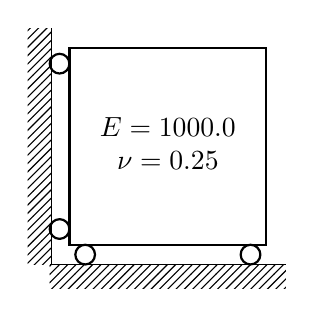
\begin{tikzpicture}[every node/.style={draw,outer sep=0pt,thick}]
  \tikzstyle{ground}=
    [fill,pattern=north east lines,
      draw=none,minimum width=0.75cm,minimum height=0.3cm]

\begin{scope}[xshift=7cm]
  % Creates the rectangle
  \node (M) [minimum width=2.5cm, minimum height=2.5cm] 
    { \makecell[c]{$E=1000.0$ \\ $\nu=0.25$} };

  % Creates the bottom ground
  \node (ground) [ground,anchor=north,yshift=-0.25cm,minimum width=3.0cm] 
          at (M.south) {};
  \draw (ground.north east) -- (ground.north west);

  % Create the bottom rollers
  \draw [thick] (M.south west) ++ ( 0.2cm,-0.125cm) circle (0.125cm)  
                (M.south east) ++ (-0.2cm,-0.125cm) circle (0.125cm);

  % Create the left ground
  \node (wall) [ground, rotate=-90, minimum width=3cm,yshift=-0.38cm]
          at (M.west) {};
  \draw (wall.north east) -- (wall.north west);

  % Create the left rollers
  \draw [thick] (M.north west) ++ (-0.125cm,-0.2cm) circle (0.125cm)  
                (M.south west) ++ (-0.125cm, 0.2cm) circle (0.125cm);
\end{scope}

\end{tikzpicture}
  \caption{Base Dirichlet boundary conditions with material 
            properties shown.}
  \label{fig:DiriBC}
\end{figure} 

Images from these three tests are shown in Sections \ref{subsec:linTris}
and \ref{subsec:quadTris} for linear and quadratic triangular
elements, respectively. 
This is then repeated for quadrilateral elements; 
results from linear quadrilateral tests are shown in 
Section \ref{subsec:linQuads}
results from quadratic quadrilateral tests are shown in 
Section \ref{subsec:quadQuads}.
Additionally, solution convergence 
is shown for the linear triangular elements 
in Section \ref{subsec:linTris} for the body loading case.
Results are presented graphically as prepared in ParaView.

\subsection{Linear Triangular Elements} \label{subsec:linTris}
The displacement results for test 1 are shown in 
Figures \ref{fig:linTri1_x} and \ref{fig:linTri1_y}.
This displacement then caused the stress distribution 
shown in Figure \ref{fig:linTri1_SXX}.
The original mesh used is shown in Figure \ref{fig:TriMesh}.
This mesh is also used for the quadratic triangular elements.

\begin{figure}[H]
  \centering
  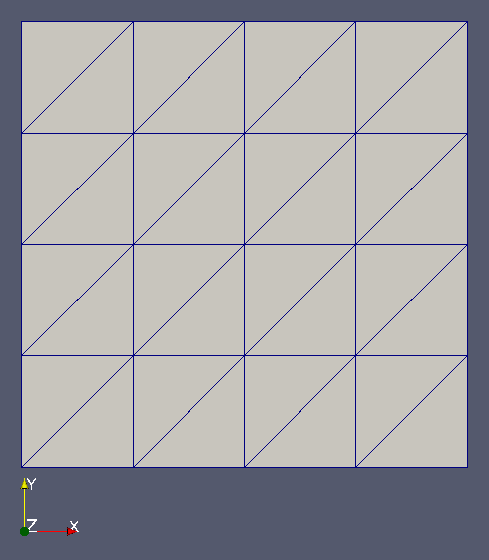
\includegraphics[width=11cm, height=11cm]{tri_4_mesh}
  \caption{Original mesh used for test 1 and 2 for the linear
            and quadratic triangular elements.}
  \label{fig:TriMesh}
\end{figure}

\begin{figure}[H]
  \centering
  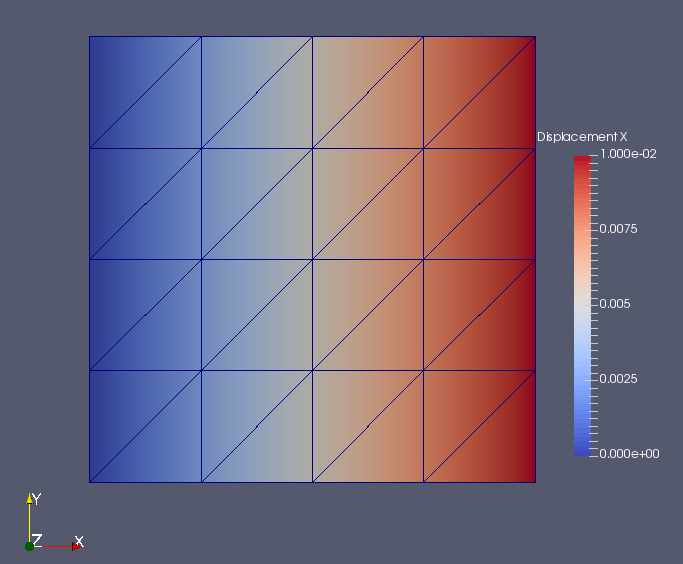
\includegraphics[width=13cm, height=10cm]{tri_4_t1_disp_X}
  \caption{Deformation X component for test 1 of linear 
            triangular elements.}
  \label{fig:linTri1_x}
\end{figure}

\begin{figure}[H]
  \centering
  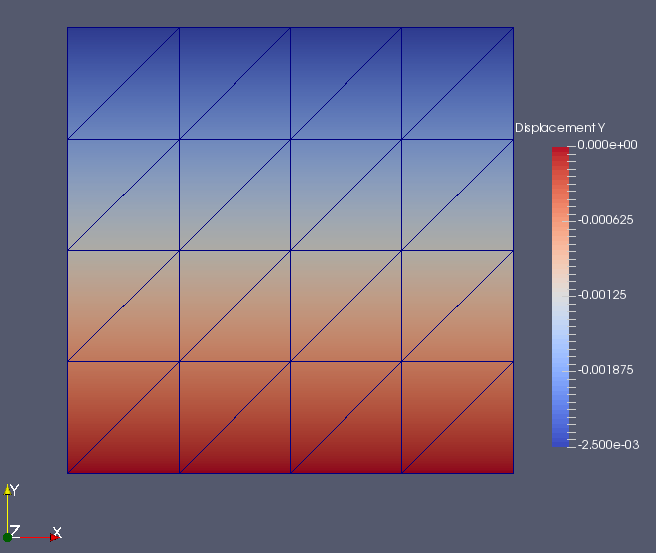
\includegraphics[width=13cm, height=10cm]{tri_4_t1_disp_Y}
  \caption{Deformation Y component for test 1 of linear 
            triangular elements.}
  \label{fig:linTri1_y}
\end{figure}

\begin{figure}[H]
  \centering
  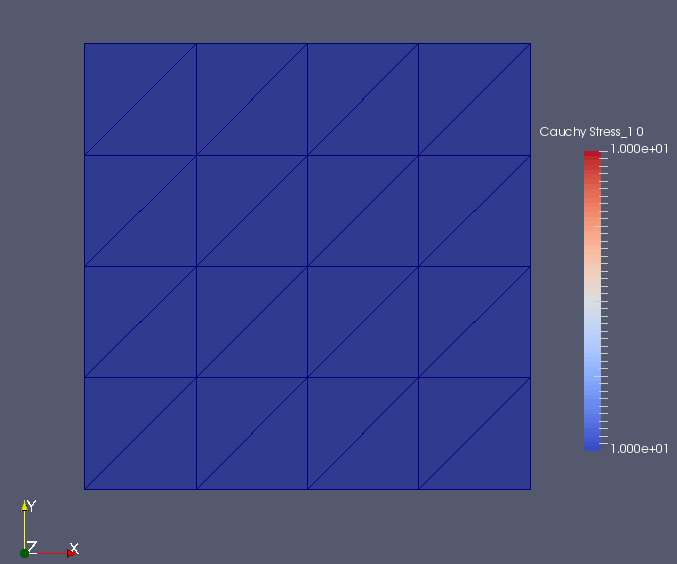
\includegraphics[width=13cm, height=10cm]{tri_4_t1_Sxx}
  \caption{The $xx$ component of the Cauchy stress for test 1.
            All other components were zero.}
  \label{fig:linTri1_SXX}
\end{figure}

The displacement results for test 2 are shown in 
Figures \ref{fig:linTri2_x} and \ref{fig:linTri2_y}.
This displacement then caused the stress distribution 
shown in Figure \ref{fig:linTri2_SXX}.

\begin{figure}[H]
  \centering
  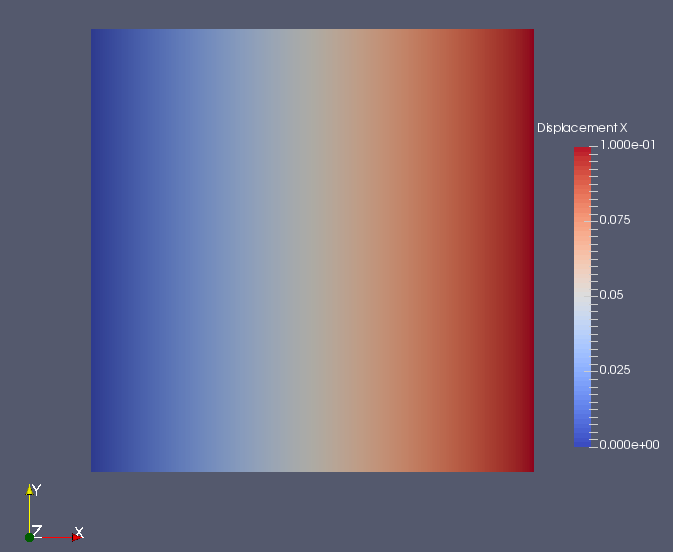
\includegraphics[width=13cm, height=10cm]{tri_4_t2_disp_X}
  \caption{Deformation X component for test 2 of linear 
            triangular elements.}
  \label{fig:linTri2_x}
\end{figure}

\begin{figure}[H]
  \centering
  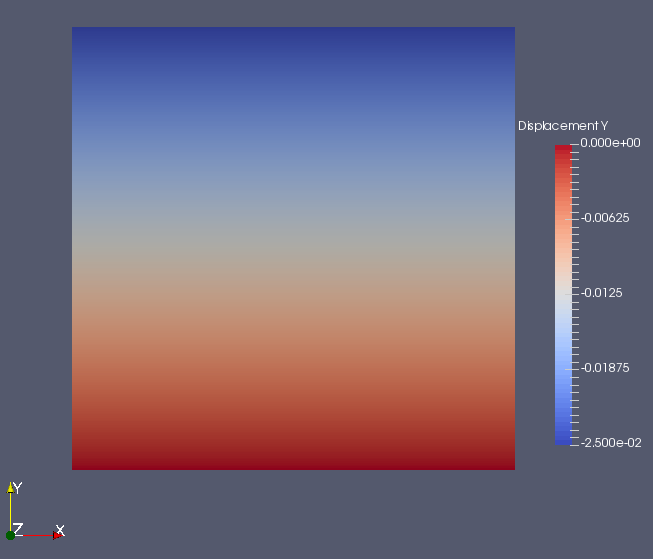
\includegraphics[width=13cm, height=10cm]{tri_4_t2_disp_Y}
  \caption{Deformation Y component for test 2 of linear 
            triangular elements.}
  \label{fig:linTri2_y}
\end{figure}

\begin{figure}[H]
  \centering
  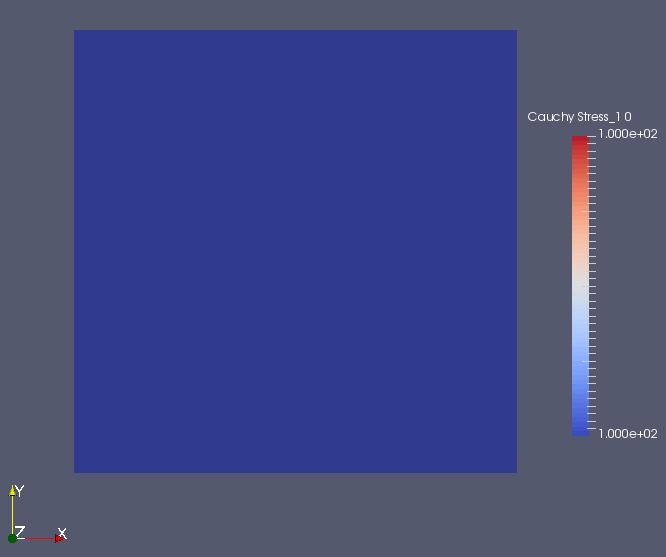
\includegraphics[width=13cm, height=10cm]{tri_4_t2_Sxx}
  \caption{The $xx$ component of the Cauchy stress for test 2.
            All other components were zero.}
  \label{fig:linTri2_SXX}
\end{figure}

The displacement results for test 3 are shown in 
Figures \ref{fig:linTri3_x} and \ref{fig:linTri3_y}.
This displacement then caused the stress distribution 
shown in Figure \ref{fig:linTri3_SXX}.

\begin{figure}[H]
  \centering
  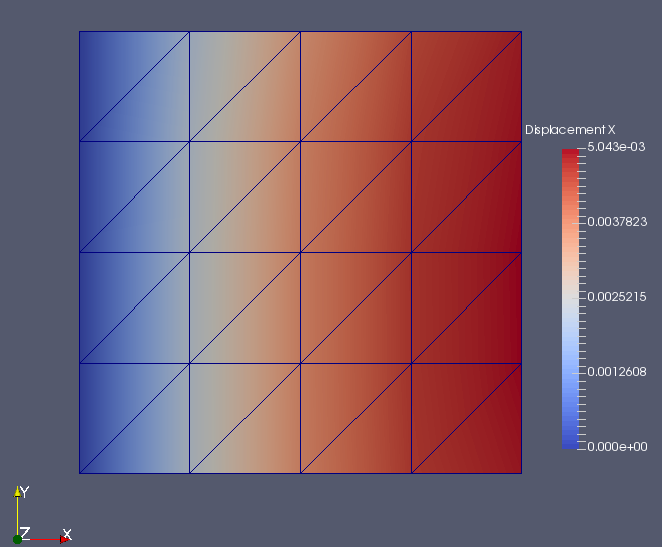
\includegraphics[width=13cm, height=10cm]{tri_4_t3_disp_X}
  \caption{Deformation X component for test 3 of linear 
            triangular elements.}
  \label{fig:linTri3_x}
\end{figure}

\begin{figure}[H]
  \centering
  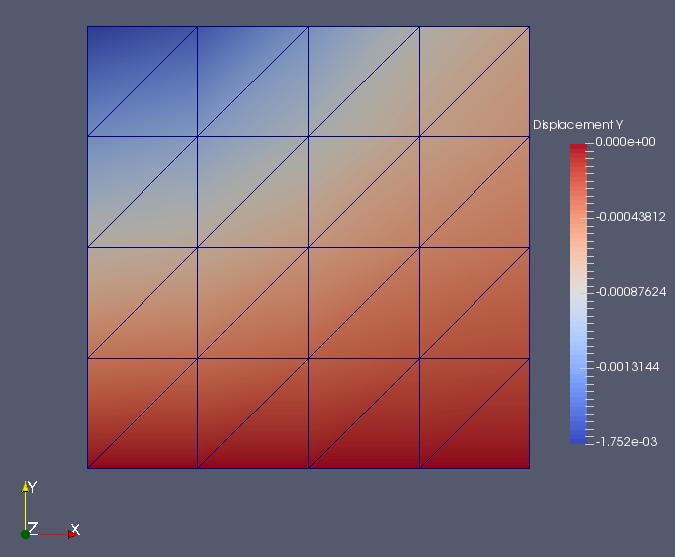
\includegraphics[width=13cm, height=10cm]{tri_4_t3_disp_Y}
  \caption{Deformation Y component for test 3 of linear 
            triangular elements.}
  \label{fig:linTri3_y}
\end{figure}

\begin{figure}[H]
  \centering
  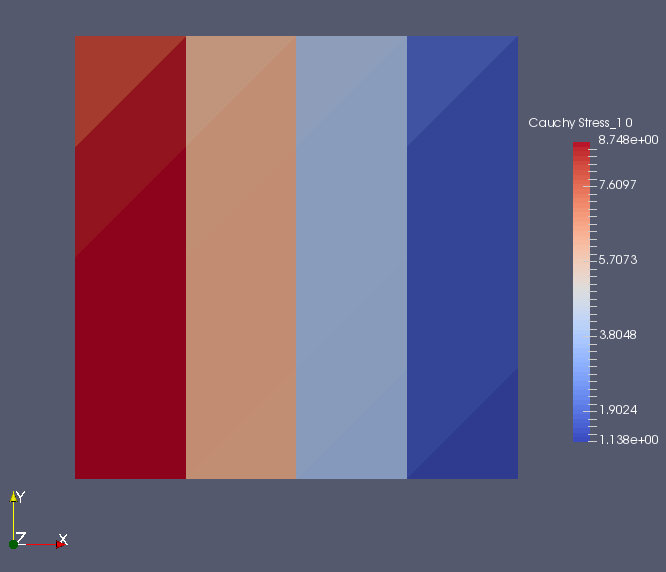
\includegraphics[width=13cm, height=10cm]{tri_4_t3_Sxx}
  \caption{The $xx$ component of the Cauchy stress for test 3.}
  \label{fig:linTri3_SXX}
\end{figure}

Convergence was also measured using test 3. This is shown in 
Figure \ref{fig:triConv}. The analytical solution for the 
body load case is shown in Equation \ref{eq:AnaSol}:

\begin{equation} \label{eq:AnaSol}
U_{a} = \frac{g(a-x_1)x_1}{E}
  \begin{bmatrix}
    1    \\
    -\nu \\
    0
  \end{bmatrix}
\end{equation}

\noindent
where $U_a$ is the analytical displacement solution, $a$ is the width
of the plate (taken as $1$ in this test), and $x_1$ is the position
along the width of the plate. The origin is taken to be the bottom
left corner.

\begin{figure}[H]
  \centering
\begin{tikzpicture}
  \begin{axis}[ 
    title=Linear Triangluar Element Convergence,
    xmode=log, 
    xlabel=$DOF$,
    ymode=log,
    ylabel=$\quad RMS$]
  \addplot table { RMS.txt };
  \end{axis}
\end{tikzpicture}
  \caption{RMS of displacement error when compared to analytical 
            solution with respect to increasing degrees of freedom.}
  \label{fig:triConv}
\end{figure}

As shown in Figure \ref{fig:triConv}, the linear triangular 
elements are able to converge on the exact, quadratic, solution
even though each element is only linear in accuracy.

\subsection{Quadratic Triangular Elements} \label{subsec:quadTris}
The displacement results for test 1 are shown in 
Figures \ref{fig:quadTri1_x} and \ref{fig:quadTri1_y}.
This displacement then caused the stress distribution 
shown in Figure \ref{fig:quadTri1_SXX}.
The original mesh used is shown in Figure \ref{fig:TriMesh}.

\begin{figure}[H]
  \centering
  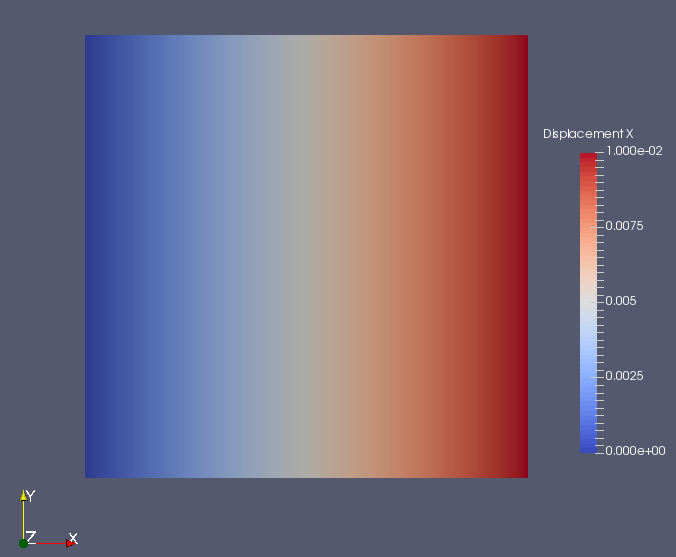
\includegraphics[width=13cm, height=10cm]{Qtri_4_t1_disp_X}
  \caption{Deformation X component for test 1 of quadratic
            triangular elements.}
  \label{fig:quadTri1_x}
\end{figure}

\begin{figure}[H]
  \centering
  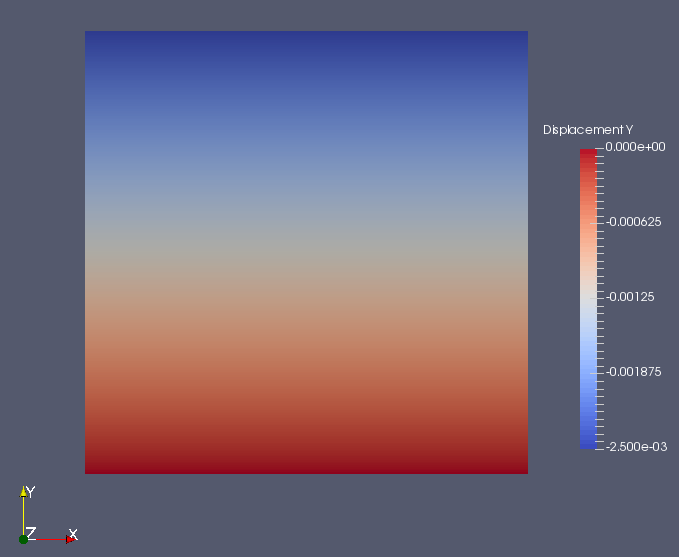
\includegraphics[width=13cm, height=10cm]{Qtri_4_t1_disp_Y}
  \caption{Deformation Y component for test 1 of quadratic
            triangular elements.}
  \label{fig:quadTri1_y}
\end{figure}

\begin{figure}[H]
  \centering
  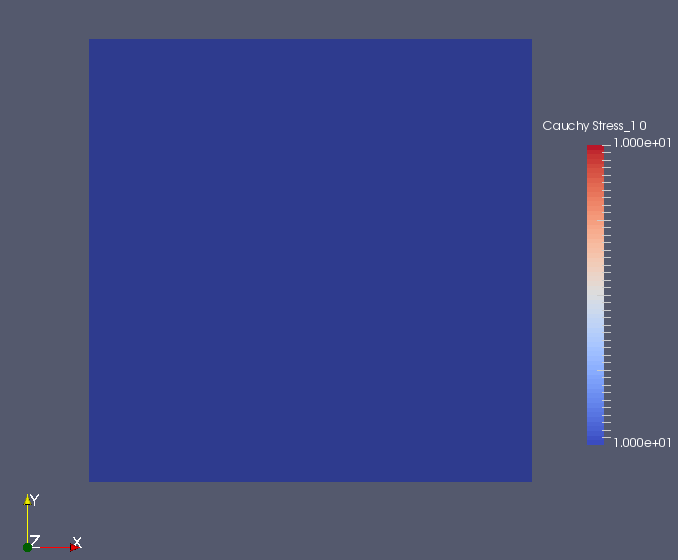
\includegraphics[width=13cm, height=10cm]{Qtri_4_t1_Sxx}
  \caption{The $xx$ component of the Cauchy stress for test 1.
            All other components were zero.}
  \label{fig:quadTri1_SXX}
\end{figure}

The displacement results for test 2 are shown in 
Figures \ref{fig:quadTri2_x} and \ref{fig:quadTri2_y}.
This displacement then caused the stress distribution 
shown in Figure \ref{fig:quadTri2_SXX}.

\begin{figure}[H]
  \centering
  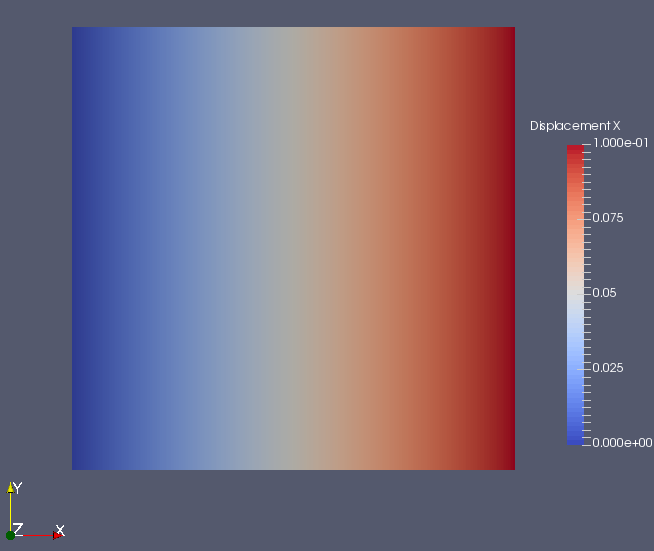
\includegraphics[width=13cm, height=10cm]{Qtri_4_t2_disp_X}
  \caption{Deformation X component for test 2 of quadratic
            triangular elements.}
  \label{fig:quadTri2_x}
\end{figure}

\begin{figure}[H]
  \centering
  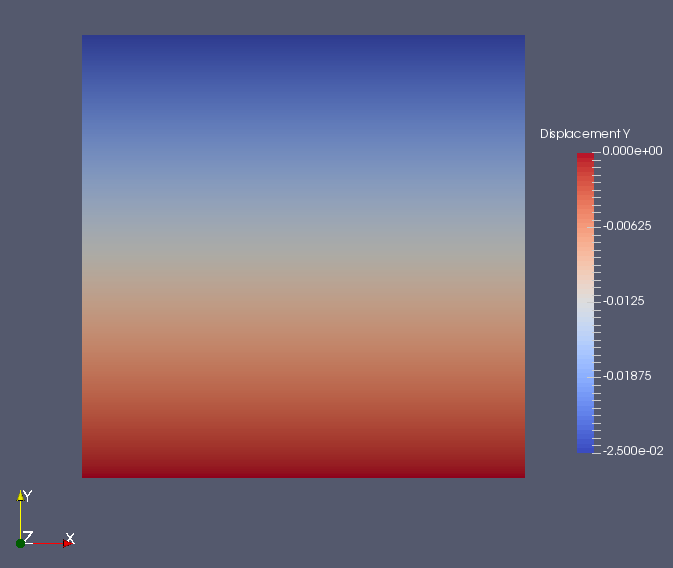
\includegraphics[width=13cm, height=10cm]{Qtri_4_t2_disp_Y}
  \caption{Deformation Y component for test 2 of quadratic
            triangular elements.}
  \label{fig:quadTri2_y}
\end{figure}

\begin{figure}[H]
  \centering
  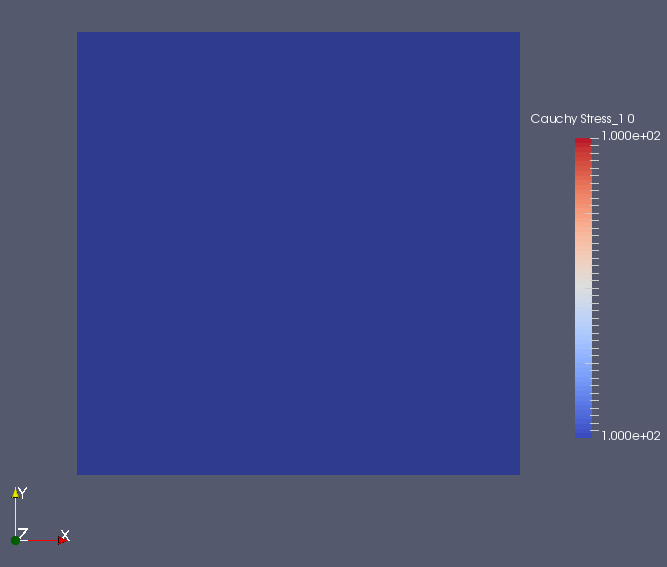
\includegraphics[width=13cm, height=10cm]{Qtri_4_t2_Sxx}
  \caption{The $xx$ component of the Cauchy stress for test 2.
            All other components were zero.}
  \label{fig:quadTri2_SXX}
\end{figure}

The displacement results for test 3 are shown in 
Figures \ref{fig:quadTri3_x} and \ref{fig:quadTri3_y}.
This displacement then caused the stress distribution 
shown in Figure \ref{fig:quadTri3_SXX}.

\begin{figure}[H]
  \centering
  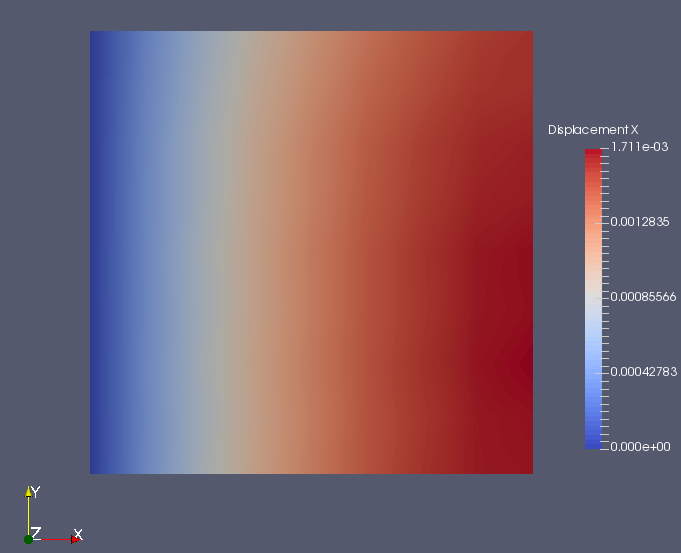
\includegraphics[width=13cm, height=10cm]{Qtri_4_t3_disp_X}
  \caption{Deformation X component for test 3 of quadratic
            triangular elements.}
  \label{fig:quadTri3_x}
\end{figure}

\begin{figure}[H]
  \centering
  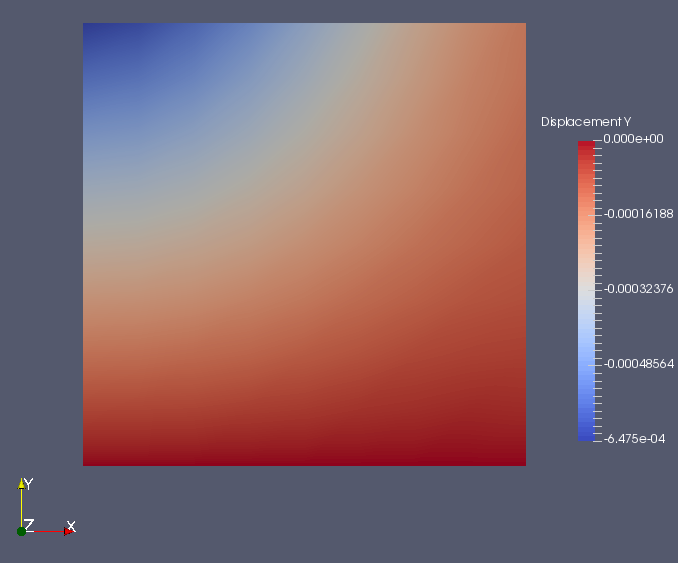
\includegraphics[width=13cm, height=10cm]{Qtri_4_t3_disp_Y}
  \caption{Deformation Y component for test 3 of quadratic
            triangular elements.}
  \label{fig:quadTri3_y}
\end{figure}

\begin{figure}[H]
  \centering
  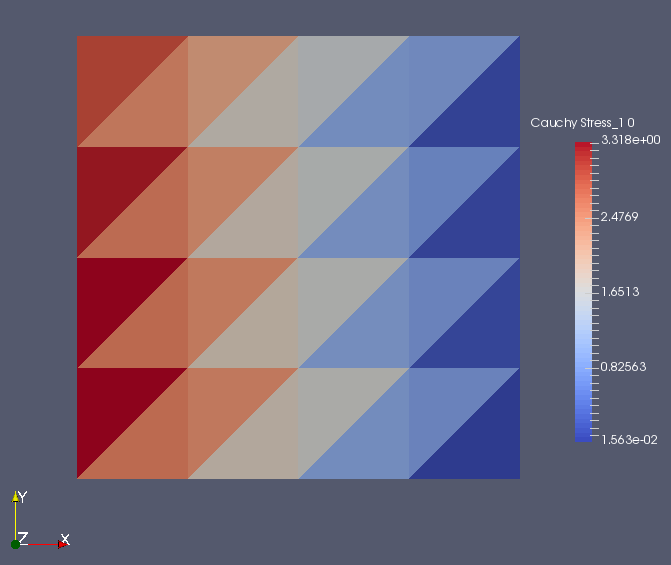
\includegraphics[width=13cm, height=10cm]{Qtri_4_t3_Sxx}
  \caption{The $xx$ component of the Cauchy stress for test 3.}
  \label{fig:quadTri3_SXX}
\end{figure}

\subsection{Linear Quadrilateral Elements} \label{subsec:linQuads}
The displacement results for test 1 are shown in 
Figures \ref{fig:linQuad1_x} and \ref{fig:linQuad1_y}.
This displacement then caused the stress distribution 
shown in Figure \ref{fig:linQuad1_SXX}.
The original mesh used is shown in Figure \ref{fig:QuadMesh}.
This mesh is also used for the quadratic quadrilateral elements.

\begin{figure}[H]
  \centering
  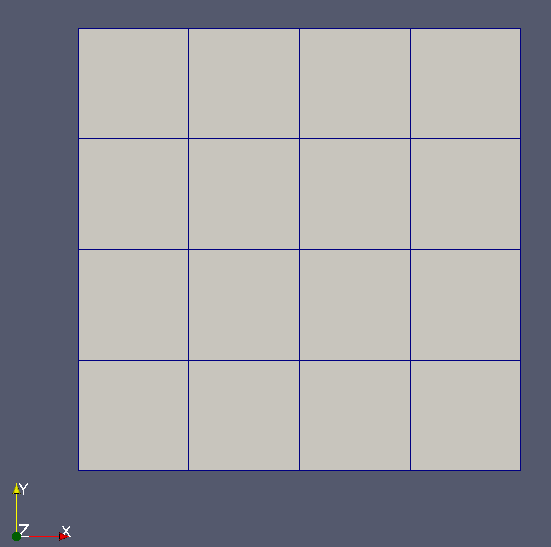
\includegraphics[width=11cm, height=11cm]{quad_4_mesh}
  \caption{Original mesh used for test 1 and 2 for the linear
            and quadratic quadrilateral elements.}
  \label{fig:QuadMesh}
\end{figure}

\begin{figure}[H]
  \centering
  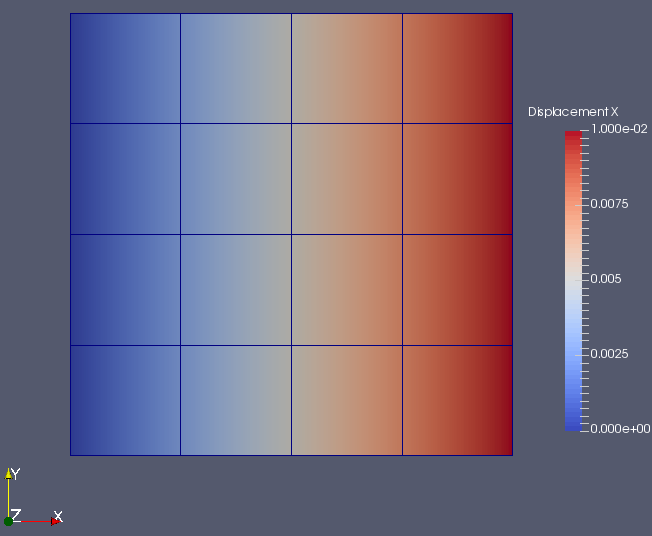
\includegraphics[width=13cm, height=10cm]{quad_4_t1_disp_X}
  \caption{Deformation X component for test 1 of linear 
            quadrilateral elements.}
  \label{fig:linQuad1_x}
\end{figure}

\begin{figure}[H]
  \centering
  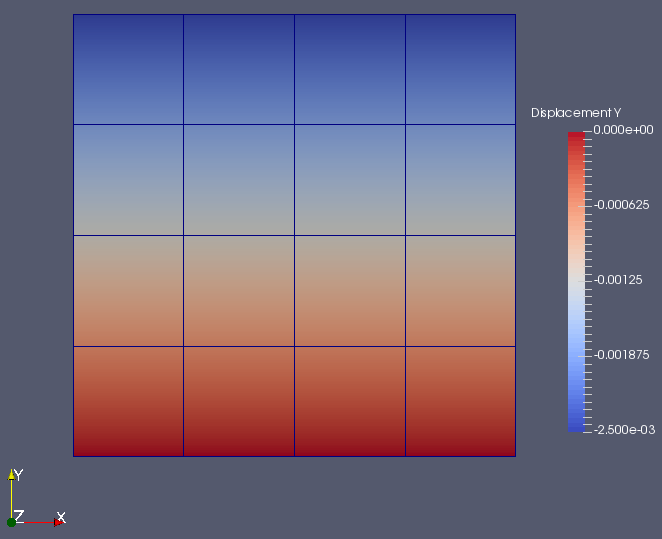
\includegraphics[width=13cm, height=10cm]{quad_4_t1_disp_Y}
  \caption{Deformation Y component for test 1 of linear 
            quadrilateral elements.}
  \label{fig:linQuad1_y}
\end{figure}

\begin{figure}[H]
  \centering
  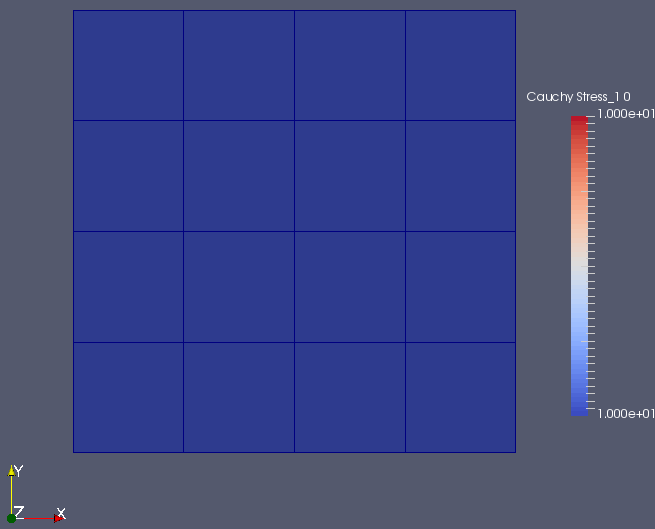
\includegraphics[width=13cm, height=10cm]{quad_4_t1_Sxx}
  \caption{The $xx$ component of the Cauchy stress for test 1.
            All other components were zero.}
  \label{fig:linQuad1_SXX}
\end{figure}

The displacement results for test 2 are shown in 
Figures \ref{fig:linQuad2_x} and \ref{fig:linQuad2_y}.
This displacement then caused the stress distribution 
shown in Figure \ref{fig:linQuad2_SXX}.

\begin{figure}[H]
  \centering
  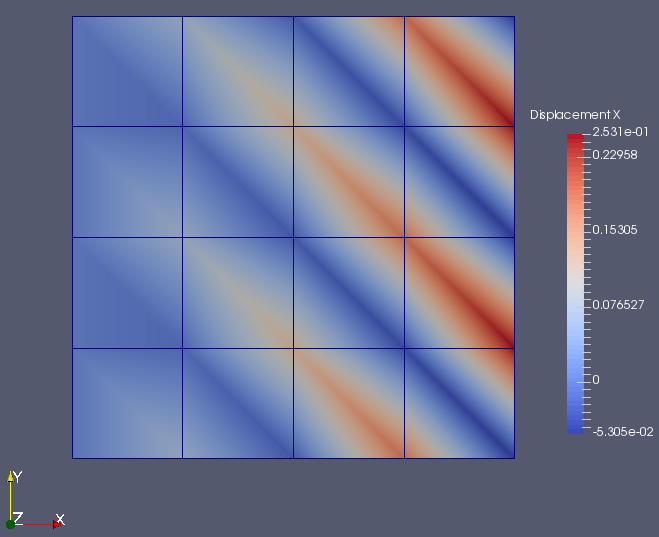
\includegraphics[width=13cm, height=10cm]{quad_4_t2_disp_X}
  \caption{Deformation X component for test 2 of linear 
            quadrilateral elements.}
  \label{fig:linQuad2_x}
\end{figure}

\begin{figure}[H]
  \centering
  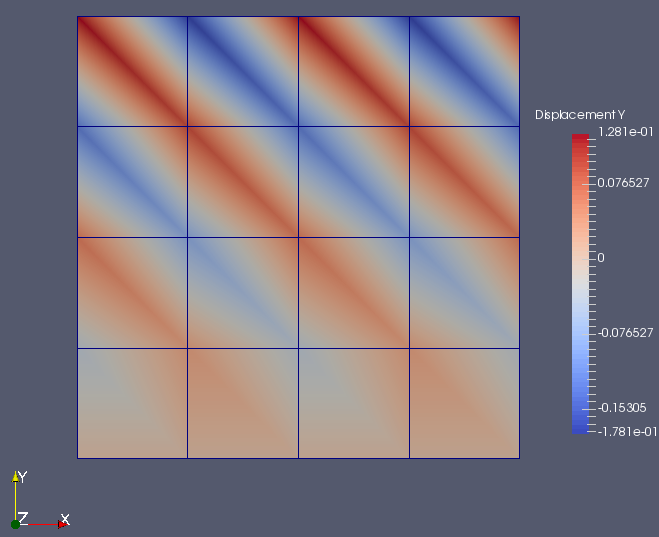
\includegraphics[width=13cm, height=10cm]{quad_4_t2_disp_Y}
  \caption{Deformation Y component for test 2 of linear 
            quadrilateral elements.}
  \label{fig:linQuad2_y}
\end{figure}

\begin{figure}[H]
  \centering
  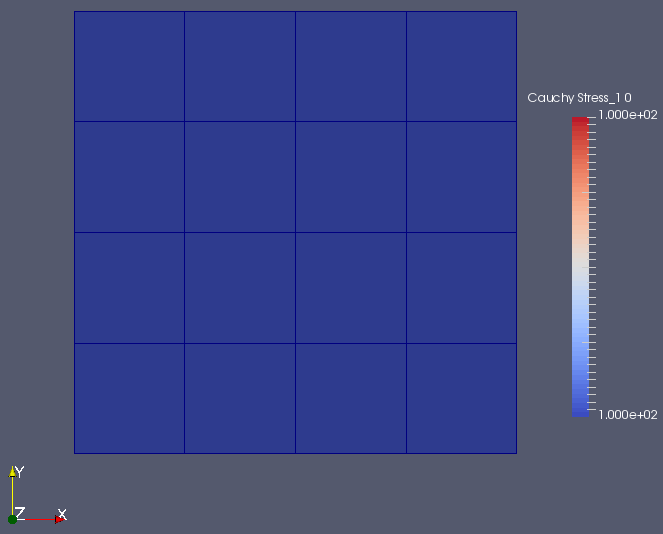
\includegraphics[width=13cm, height=10cm]{quad_4_t2_Sxx}
  \caption{The $xx$ component of the Cauchy stress for test 2.
            All other components were zero.}
  \label{fig:linQuad2_SXX}
\end{figure}

The displacement results for test 3 are shown in 
Figures \ref{fig:linQuad3_x} and \ref{fig:linQuad3_y}.
This displacement then caused the stress distribution 
shown in Figure \ref{fig:linQuad3_SXX}.

\begin{figure}[H]
  \centering
  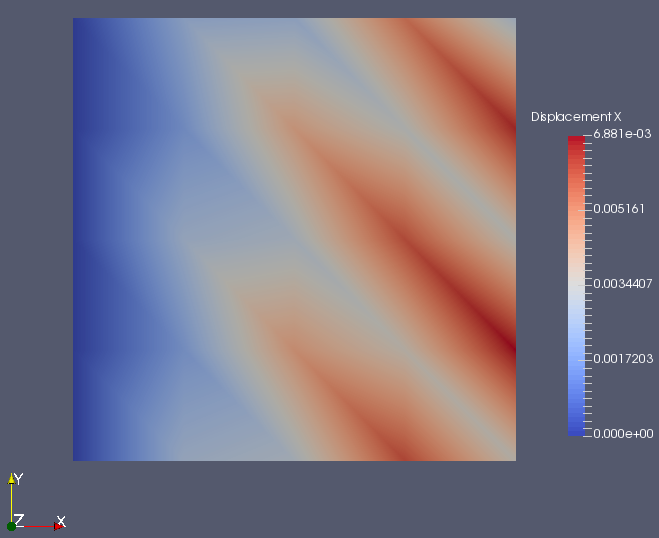
\includegraphics[width=13cm, height=10cm]{quad_4_t3_disp_X}
  \caption{Deformation X component for test 3 of linear 
            quadrilateral elements.}
  \label{fig:linQuad3_x}
\end{figure}

\begin{figure}[H]
  \centering
  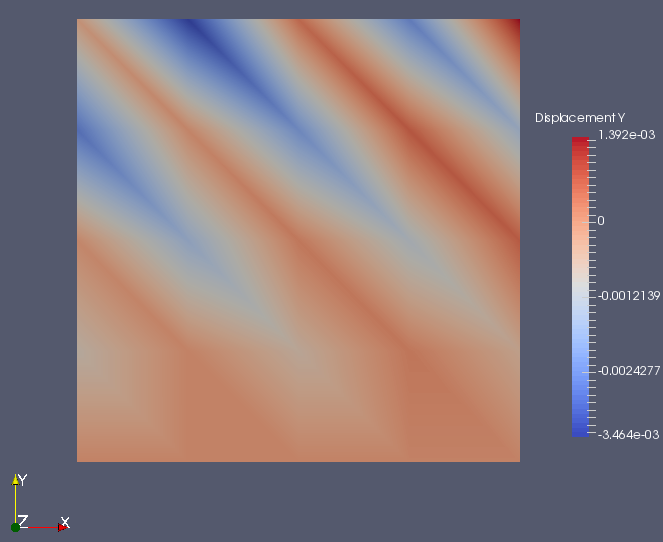
\includegraphics[width=13cm, height=10cm]{quad_4_t3_disp_Y}
  \caption{Deformation Y component for test 3 of linear 
            quadrilateral elements.}
  \label{fig:linQuad3_y}
\end{figure}

\begin{figure}[H]
  \centering
  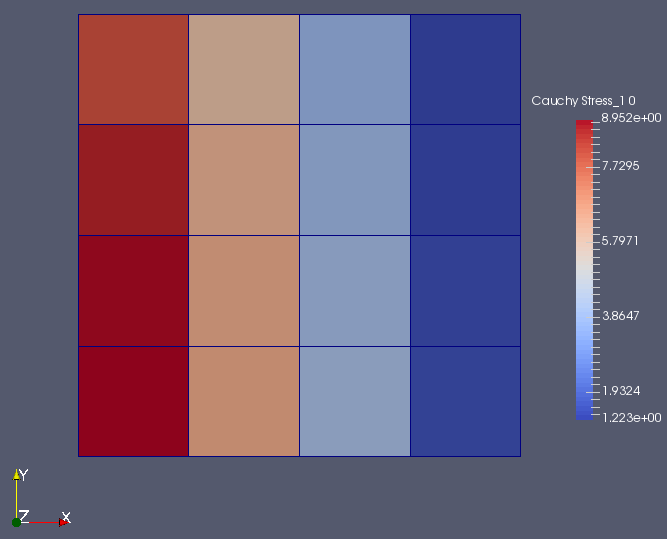
\includegraphics[width=13cm, height=10cm]{quad_4_t3_Sxx}
  \caption{The $xx$ component of the Cauchy stress for test 3.}
  \label{fig:linQuad3_SXX}
\end{figure}

\subsection{Quadratic Quadrilaterals Elements} \label{subsec:quadQuads}
The displacement results for test 1 are shown in 
Figures \ref{fig:quadQuad1_x} and \ref{fig:quadQuad1_y}.
This displacement then caused the stress distribution 
shown in Figure \ref{fig:quadQuad1_SXX}.
The original mesh used is shown in Figure \ref{fig:QuadMesh}.

\begin{figure}[H]
  \centering
  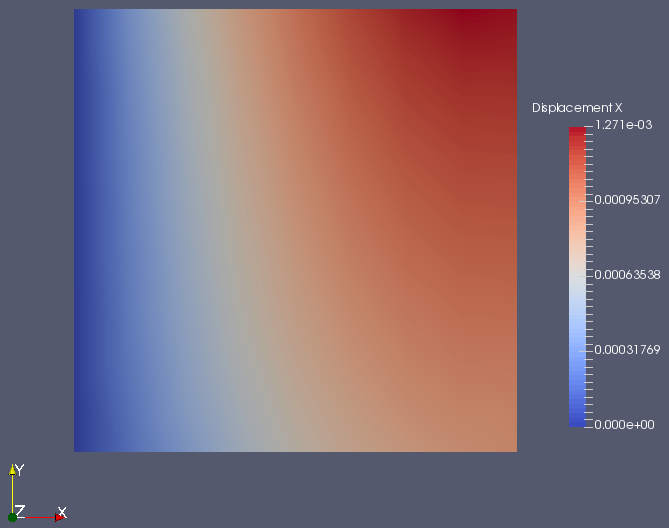
\includegraphics[width=13cm, height=10cm]{Qquad_4_t1_disp_X}
  \caption{Deformation X component for test 1 of quadratic
            quadrilateral elements.}
  \label{fig:quadQuad1_x}
\end{figure}

\begin{figure}[H]
  \centering
  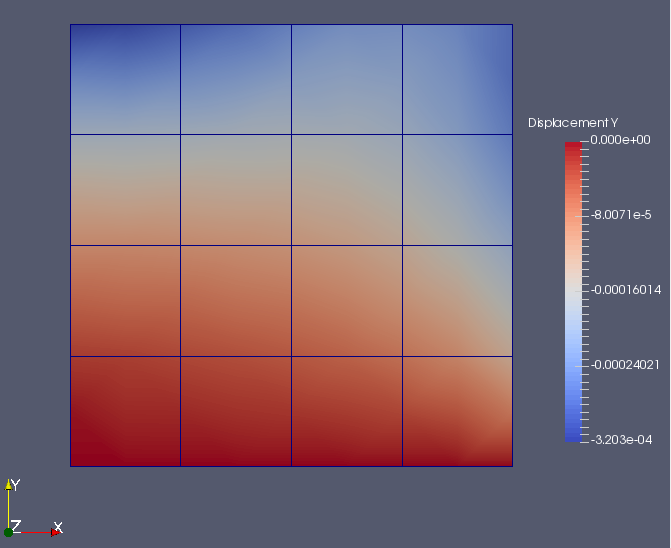
\includegraphics[width=13cm, height=10cm]{Qquad_4_t1_disp_Y}
  \caption{Deformation Y component for test 1 of quadratic
            quadrilateral elements.}
  \label{fig:quadQuad1_y}
\end{figure}

\begin{figure}[H]
  \centering
  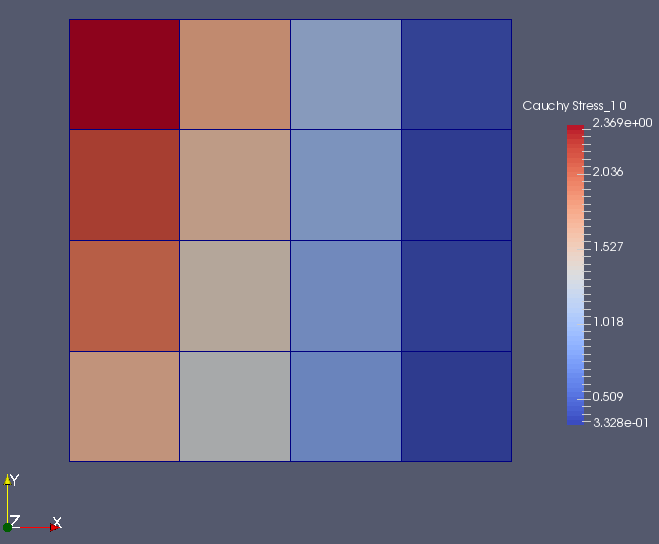
\includegraphics[width=13cm, height=10cm]{Qquad_4_t1_Sxx}
  \caption{The $xx$ component of the Cauchy stress for test 1.
            All other components were zero.}
  \label{fig:quadQuad1_SXX}
\end{figure}

The displacement results for test 2 are shown in 
Figures \ref{fig:quadQuad2_x} and \ref{fig:quadTri2_y}.
This displacement then caused the stress distribution 
shown in Figure \ref{fig:quadQuad2_SXX}.

\begin{figure}[H]
  \centering
  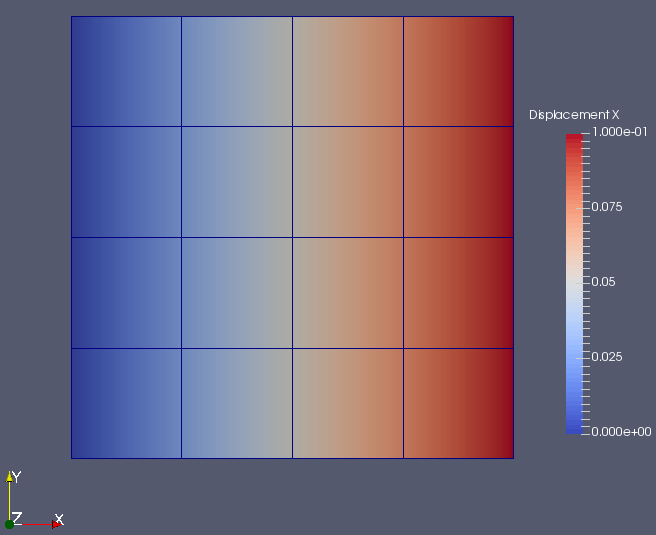
\includegraphics[width=13cm, height=10cm]{Qquad_4_t2_disp_X}
  \caption{Deformation X component for test 2 of quadratic
            quadrilateral elements.}
  \label{fig:quadQuad2_x}
\end{figure}

\begin{figure}[H]
  \centering
  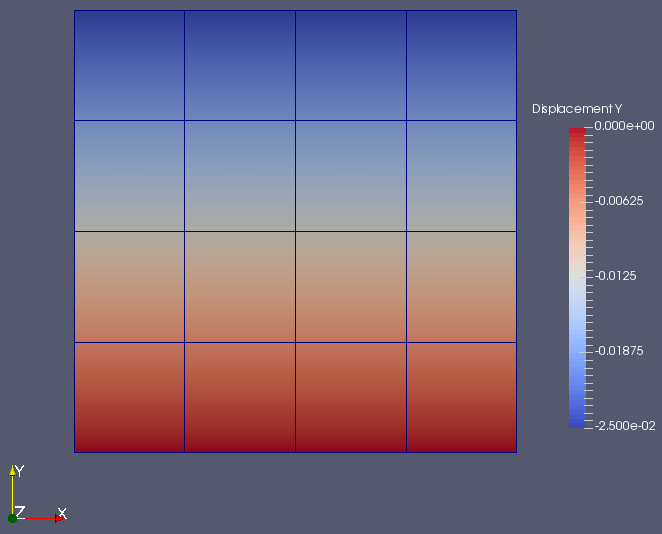
\includegraphics[width=13cm, height=10cm]{Qquad_4_t2_disp_Y}
  \caption{Deformation Y component for test 2 of quadratic
            quadrilateral elements.}
  \label{fig:quadQuad2_y}
\end{figure}

\begin{figure}[H]
  \centering
  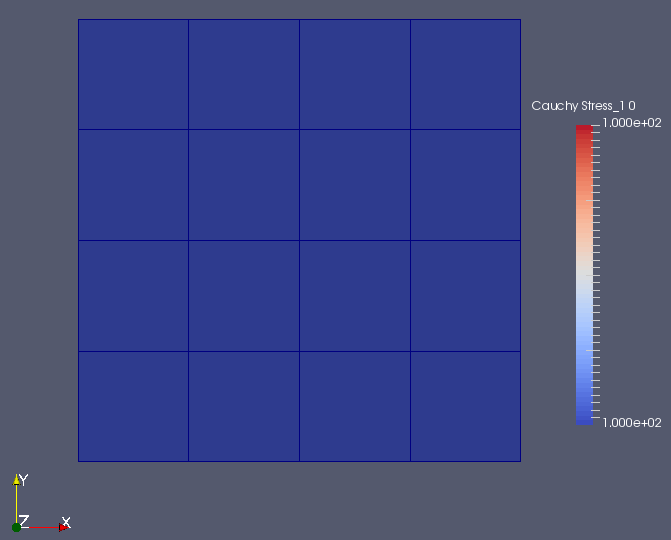
\includegraphics[width=13cm, height=10cm]{Qquad_4_t2_Sxx}
  \caption{The $xx$ component of the Cauchy stress for test 2.
            All other components were zero.}
  \label{fig:quadQuad2_SXX}
\end{figure}

The displacement results for test 3 are shown in 
Figures \ref{fig:quadQuad3_x} and \ref{fig:quadTri3_y}.
This displacement then caused the stress distribution 
shown in Figure \ref{fig:quadQuad3_SXX}.

\begin{figure}[H]
  \centering
  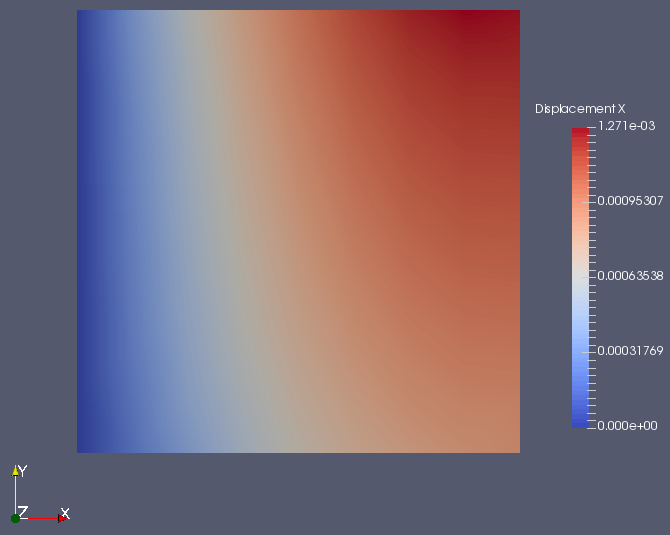
\includegraphics[width=13cm, height=10cm]{Qquad_4_t3_disp_X}
  \caption{Deformation X component for test 3 of quadratic
            quadrilateral elements.}
  \label{fig:quadQuad3_x}
\end{figure}

\begin{figure}[H]
  \centering
  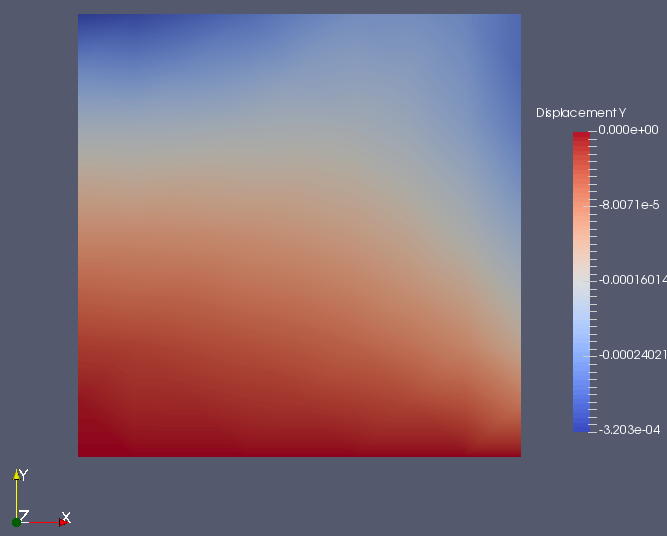
\includegraphics[width=13cm, height=10cm]{Qquad_4_t3_disp_Y}
  \caption{Deformation Y component for test 3 of quadratic
            quadrilateral elements.}
  \label{fig:quadQuad3_y}
\end{figure}

\begin{figure}[H]
  \centering
  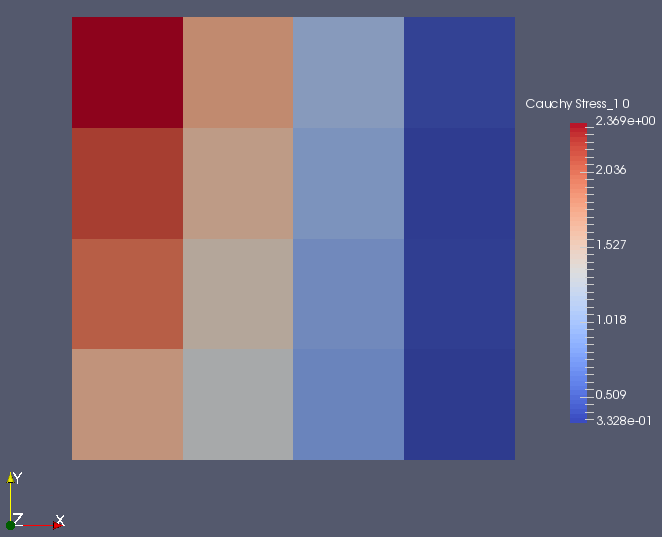
\includegraphics[width=13cm, height=10cm]{Qquad_4_t3_Sxx}
  \caption{The $xx$ component of the Cauchy stress for test 3.}
  \label{fig:quadQuad3_SXX}
\end{figure}

\section{Conclusion} \label{sec:conclusion}
The purpose of this project was to develop a FEA code that 
solves linear elliptic problems. This project did so for
two dimensional plane stress solid mechanic problems. 

The code presented would be able to solve similar two 
dimensional problems if needed. For example, plane strain 
problems could be evaluated by adjusting the material tensor $D$
in the elemental stiffness integrator. 
The user provides the problem statement via geometric definition.
This is shown by use of the \texttt{.yaml} and \texttt{associations}
file; the user specifies collections of model entities on which 
boundary conditions are applied.
The code is able to use either triangular or
quadrilateral elements. It can also can use
either first or second order shape functions and numerical integration
schemes at the user's discretion.
When building the linear system, the code uses the compressed
row storage methods provided by the \texttt{Trilinos} 
software framework; the system is then solved using the GMRES 
method provided by the same framework.
Once the solution, displacement components at the nodes, 
is recovered the secondary variable, stress, is also calculated.
Both of these quantities are then output graphically in the 
form of Vtk files.

\subsection{Closing Comments} \label{sec:comments}
The displacement fields shown for the linear quadrilateral 
elements in Figures 
\ref{fig:linQuad2_x}, \ref{fig:linQuad2_y}, 
\ref{fig:linQuad3_x}, and  \ref{fig:linQuad3_y} are wrong 
as they do not make any physical sense. 
I wasn't able to figure out what was causing this; especially 
since the quadratic quadrilaterals worked as expected.

A better convergence study would have been to measure the
stress magnification factor for a sufficiently large 
plate with a circular hole. This would have shown the 
convergence rates for each element combination independently 
as they approach the theoretical value of 3.

\newpage
\appendix
\section{Source Code and Headers} \label{sec:code}

\subsection{a4.cc} \label{subsec:a4.cc}
\lstinputlisting{/lore/clougj/FiniteElementProgramming/a4/src/a4.cc}

\newpage
\subsection{A4\_BodyLoads.hpp} \label{subsec:BLhpp}
\lstinputlisting{/lore/clougj/FiniteElementProgramming/a4/src/A4_BodyLoads.hpp}

\newpage
\subsection{A4\_BodyLoads.cpp} \label{subsec:BLcpp}
\lstinputlisting{/lore/clougj/FiniteElementProgramming/a4/src/A4_BodyLoads.cpp}

\newpage
\subsection{A4\_Control.hpp} \label{subsec:Cont.hpp}
\lstinputlisting{/lore/clougj/FiniteElementProgramming/a4/src/A4_Control.hpp}

\newpage
\subsection{A4\_Control.cpp} \label{subsec:Cont.cpp}
\lstinputlisting{/lore/clougj/FiniteElementProgramming/a4/src/A4_Control.cpp}

\newpage
\subsection{A4\_DBCs.hpp} \label{subsec:DBCs.hpp}
\lstinputlisting{/lore/clougj/FiniteElementProgramming/a4/src/A4_DBCs.hpp}

\newpage
\subsection{A4\_DBCs.cpp} \label{subsec:DBCs.cpp}
\lstinputlisting{/lore/clougj/FiniteElementProgramming/a4/src/A4_DBCs.cpp}

\newpage
\subsection{A4\_Disc.hpp} \label{subsec:Disc.hpp}
\lstinputlisting{/lore/clougj/FiniteElementProgramming/a4/src/A4_Disc.hpp}

\newpage
\subsection{A4\_Disc.cpp} \label{subsec:Disc.cpp}
\lstinputlisting{/lore/clougj/FiniteElementProgramming/a4/src/A4_Disc.cpp}

\newpage
\subsection{A4\_ElasticStiffness.hpp} \label{subsec:ElasticStiffness.hpp}
\lstinputlisting{/lore/clougj/FiniteElementProgramming/a4/src/A4_ElasticStiffness.hpp}

\newpage
\subsection{A4\_ElasticStiffness.cpp} \label{subsec:ElasticStiffness.cpp}
\lstinputlisting{/lore/clougj/FiniteElementProgramming/a4/src/A4_ElasticStiffness.cpp}

\newpage
\subsection{A4\_FESolver.hpp} \label{subsec:FESolver.hpp}
\lstinputlisting{/lore/clougj/FiniteElementProgramming/a4/src/A4_FESolver.hpp}

\newpage
\subsection{A4\_FESolver.cpp} \label{subsec:FESolver.cpp}
\lstinputlisting{/lore/clougj/FiniteElementProgramming/a4/src/A4_FESolver.cpp}

\newpage
\subsection{A4\_LinAlg.hpp} \label{subsec:LinAlg.hpp}
\lstinputlisting{/lore/clougj/FiniteElementProgramming/a4/src/A4_LinAlg.hpp}

\newpage
\subsection{A4\_LinAlg.cpp} \label{subsec:LinAlg.cpp}
\lstinputlisting{/lore/clougj/FiniteElementProgramming/a4/src/A4_LinAlg.cpp}

\newpage
\subsection{A4\_LinSolve.hpp} \label{subsec:LinSolve.hpp}
\lstinputlisting{/lore/clougj/FiniteElementProgramming/a4/src/A4_LinSolve.hpp}

\newpage
\subsection{A4\_LinSolve.cpp} \label{subsec:LinSolve.cpp}
\lstinputlisting{/lore/clougj/FiniteElementProgramming/a4/src/A4_LinSolve.cpp}

\newpage
\subsection{A4\_NBCs.hpp} \label{subsec:NBCs.hpp}
\lstinputlisting{/lore/clougj/FiniteElementProgramming/a4/src/A4_NBCs.hpp}

\newpage
\subsection{A4\_NBCs.cpp} \label{subsec:NBCs.cpp}
\lstinputlisting{/lore/clougj/FiniteElementProgramming/a4/src/A4_NBCs.cpp}

\newpage
\subsection{A4\_PostProc.hpp} \label{subsec:PostProc.hpp}
\lstinputlisting{/lore/clougj/FiniteElementProgramming/a4/src/A4_PostProc.hpp}

\newpage
\subsection{A4\_PostProc.cpp} \label{subsec:PostProc.cpp}
\lstinputlisting{/lore/clougj/FiniteElementProgramming/a4/src/A4_PostProc.cpp}

\newpage
\section{Example Input and Control Files}\label{sec:ExInput}

\subsection{Associations File} \label{subsec:ExAssoc}
The associations files followed the following format:
\newline
$\{Set\_Type\} \quad  \{Name\} \quad  \{Number\_of\_Model\_Entites\} \quad $
\newline
$\{Model\_Entity\_Order\} \quad  \{Model\_Entity\_Tag\_Number\} \quad $
\newline
$\{Model\_Entity\_Order\} \quad  \{Model\_Entity\_Tag\_Number\} \quad $
\newline
$\vdots$
\newline
$\{Model\_Entity\_Order\} \quad  \{Model\_Entity\_Tag\_Number\} \quad $
\newline
$\{Set\_Type\} \quad  \{Name\} \quad  \{Number\_of\_Model\_Entites\} \quad $
\newline
$\vdots$
\newline
\lstinputlisting{/lore/clougj/FiniteElementProgramming/a4/test/plane2D.txt}

\newpage
\subsection{Example .yaml File} \label{subsec:ExYaml}
\lstinputlisting{/lore/clougj/FiniteElementProgramming/a4/test/fem.yaml}

\newpage
\subsection{Example Input Script} \label{subsec:ExIn}
\lstinputlisting{/lore/clougj/FiniteElementProgramming/a4/test/run_test.sh}

\newpage
\section{Derivations} \label{sec:Derivations}

Nomenclature for all equations shown in this section
matches that described in the main body of this report.
See Section \ref{sec:techDes} for variable descriptions.

\subsection{Strong to Weak Form Derivation} \label{sec:WeakDer}

Given:
\begin{equation*}
\sigma_{ij},_{j} - f_{i} = 0 \quad \text{and} \quad
w_{i} \in H^1, w_{i}\Big|_{\Gamma^{g}_{i}} = 0
    \quad \forall \quad i=1(1)n_{sd}
\end{equation*}

\begin{equation*}
\sigma_{ij},_{j} = c_{ijkm} \varepsilon_{km} = c_{ijkm} u_{k},_{m}
\end{equation*}

\noindent
Solution:

\begin{align*}
\int_{\Omega} w_{i} c_{ijkm} u_{k},_{mj} d\Omega -
  \int_{\Omega} w_{i} f_{i} d\Omega &= 0 \\
-c_{ijkm}(w_{i} u_{k},_{mj})\Big|_{\partial\Omega = \Gamma}
  + \int_{\Omega} c_{ijkm} w_{i},_{j} u_{k},_{m} d\Omega
  &=\int_{\Omega} w_{i} f_{i} d\Omega  \\
-c_{ijkm}(w_{i} u_{k},_{mj})\Big|_{\Gamma^{g}_{i}}
-c_{ijkm}(w_{i} u_{k},_{mj})\Big|_{\Gamma^{h}_{i}}
  + \int_{\Omega} c_{ijkm} w_{i},_{j} u_{k},_{m} d\Omega
  &=\int_{\Omega} w_{i} f_{i} d\Omega \\
0
 -c_{ijkm}(w_{i} u_{k},_{mj})\Big|_{\Gamma^{h}_{i}}
  + \int_{\Omega} c_{ijkm} w_{i},_{j} u_{k},_{m} d\Omega
  &=\int_{\Omega} w_{i} f_{i} d\Omega \\
-w_{i}\Big|_{\Gamma^{h}_{i}} h_{i}
  + \int_{\Omega} c_{ijkm} w_{i},_{j} u_{k},_{m} d\Omega
  &=\int_{\Omega} w_{i} f_{i} d\Omega \\
\int_{\Omega} c_{ijkm} w_{i},_{j} u_{k},_{m} d\Omega &=
  \int_{\Omega} w_{i} f_{i} d\Omega +
  w_{i}\Big|_{\Gamma^{h}_{i}} h_{i}
\end{align*}

\newpage
\subsection{Weak to Galerkin Form Derivation} \label{sec:GalerkinDer}

Given:
\begin{align*}
a( X, Y ) &=
  \int_{\Omega} c_{ijkm} X_{i},_{j} Y_{k},_{m} d\Omega \\
b( X, Y ) &=
  \int_{\Omega} X_{i} Y_{i} d\Omega \\
u^{h}_{i} =
  v^{h}_{i} + g^{h}_{i}
  \quad
  g^{h}_{i}\Big|_{\Gamma^{g}_{i}} &= g_{i}
  \quad
  v^{h}_{i}\Big|_{\Gamma^{g}_{i}} = 0
\end{align*}

\noindent
Solution:

\begin{align*}
\int_{\Omega} c_{ijkm} w_{i},_{j} u_{k},_{m} d\Omega
 &= \int_{\Omega} w_{i} f_{i} d\Omega
  + w_{i}\Big|_{\Gamma^{h}_{i}} h_{i} \\
a(w, u)
 &= b(w , f)
  + w_{i}\Big|_{\Gamma^{h}_{i}} h_{i}  \\
\text{let} \quad u &\approx u^{h} = v^{h} + g^{h} \\
 \quad w &\approx w^{h} \\
a(w^{h} , u^{h} )
 &= b(w^{h}, f)
  + w^{h}_{i}\Big|_{\Gamma^{h}_{i}} h_{i}  \\
a(w^{h} , v^{h} )
  + a(w^{h} , g^{h} )
 &= b(w^{h}, f)
  + w^{h}_{i}\Big|_{\Gamma^{h}_{i}} h_{i}  \\
a(w^{h} , v^{h})
 &= b(w^{h} , f)
  + w^{h}_{i}\Big|_{\Gamma^{h}_{i}} h_{i}
  - a(w^{h} , g^{h})
\end{align*}

\newpage
\subsection{Galerkin to Matrix Form Derivation} \label{sec:MatrixDer}

Given:
\begin{equation*}
a(w^{h} , v^{h})
 = b(w^{h} , f)
  + w^{h}_{i}\Big|_{\Gamma^{h}_{i}} h_{i}
  - a(w^{h} , g^{h})
\end{equation*}

\begin{align*}
w^{h}_i &= \sum_{A=1}^{n} c^{A}_i N^{A}  \\
v^{h}_i &= \sum_{A=1}^{n} d^{A}_i N^{A}  \\
g^{h}_i &=  \sum_{A=1}^{n} g^{A}_i N^{A}
\end{align*}

\noindent
Solution:

\begin{equation*}
a(c^{A} N^{A}, d^{B} N^{B})
 = b( c^{A} N^{A} , f)
  + c^{A} N^{A}\Big|_{\Gamma^{h}_{i}} h_{i}
  - a( c^{A} N^{A}, g^{C} N^{C})
\end{equation*}

\begin{equation*}
c^{A} a(N^{A}, N^{B})d^{B}
 = c^{A} b( N^{A} , f)
  + c^{A} N^{A}\Big|_{\Gamma^{h}_{i}} h_{i}
  - c^{A}a( N^{A}, N^{C})g^{C}
\end{equation*}

\begin{equation*}
a(N^{A}, N^{B})d^{B}
 = b( N^{A} , f)
  + N^{A}\Big|_{\Gamma^{h}_{i}} h_{i}
  - a( N^{A}, N^{C})g^{C}
\end{equation*}

\begin{align*}
\text{Let}\quad K_{AB} &= a(N^{A}, N^{B}) \\
F_A &= b( N^{A} , f)
  + N^{A}\Big|_{\Gamma^{h}_{i}} h_{i}
  - a( N^{A}, N^{C})g^{C}
\end{align*}

\begin{equation*}
[ K_{AB} ] \{ d_B \} = \{ F_A \}
\end{equation*}

\end{document}
